\chapter{Experiments}
\label{sec:experiments}
We did several experiments to answer the following questions:
\begin{enumerate}
    \item How stable is the cycle count per iteration?
    \item Is there any overhead for more \acp{pe}?
    \item When using a fixed grid size, how does the performance of using more \acp{pe} compare to using larger tiles on fewer \acp{pe}?
    \item What is the maximum tiling size that fits into the memory of a \ac{pe}?
    \item How does the performance of the generalized algorithm compare to the specialized algorithm for radius 1?
    \item How does the Cerebras implementation compare to highly optimized implementations on traditional \ac{hpc}-Arcitectures (\ac{cpu}, \ac{gpu})?
    \item What percentage of the peak performance is achieved for different tile sizes and radii?
    % \item What contributes to the cycle count?
\end{enumerate}

All experiments are performed on the cycle accurate simulator that is part of the Cerebras \ac{sdk} of which we used the version 1.3.0.
Using the simulator limits the number of \acp{pe} and number of iterations so that the data needs to be extrapolated to the whole grid.
We examine to what extend extrapolation is possible in the first two experiments.

We count the cycles used per iteration in the simulator and use this together with the clock speed of the \ac{wse} to calculate the time per iteration.

One difference between the simulator and the real hardware is that the simulator does use a single clock for all cores, while the real hardware has a separate clock for each core. (verify this!!!) Because these clocks are not perfectly synchronized, especially experiments with a large number of \acp{pe} could differ in the cycle count. Although this is not guaranteed for our algorithm, (source) find that in practice the slighly desynchronized clocks improve overall performance compared to the simulator. 

\section{Stability of cycle count per iteration}
For this experiment, we fix the grid size, tile size and radius and run the simulation for different number of iterations.
After two iterations of varying cycle count, the cycle is mostly stable.
For a grid size of 10x10, the cycle count per iteration is $16\pm1$ on \ac{wse}-2 and $23\pm1$ on \ac{wse}-3.

For a grid of 10x10, and a tile size of 1x1 and radius 1, the tiled algorithm achives $127\pm0$ cycles per iteration on \ac{wse}-2 and $156\pm1$ cycles per iteration on \ac{wse}-3.

A larger problem size with a grid of 100x100, tile size of 10x10 and radius 5, results in a cycle count per iteration of $3353\pm20$ on \ac{wse}-2 and $3377\pm5$ on \ac{wse}-3.

Because of the high flucuations in the cycle count in the first two iterations, we measure the cycle count in the following experiments as an average of the 3rd and 4th iteration.

\begin{figure}[h]
    \centering
    \begin{subfigure}[b]{0.48\textwidth}
        \centering
        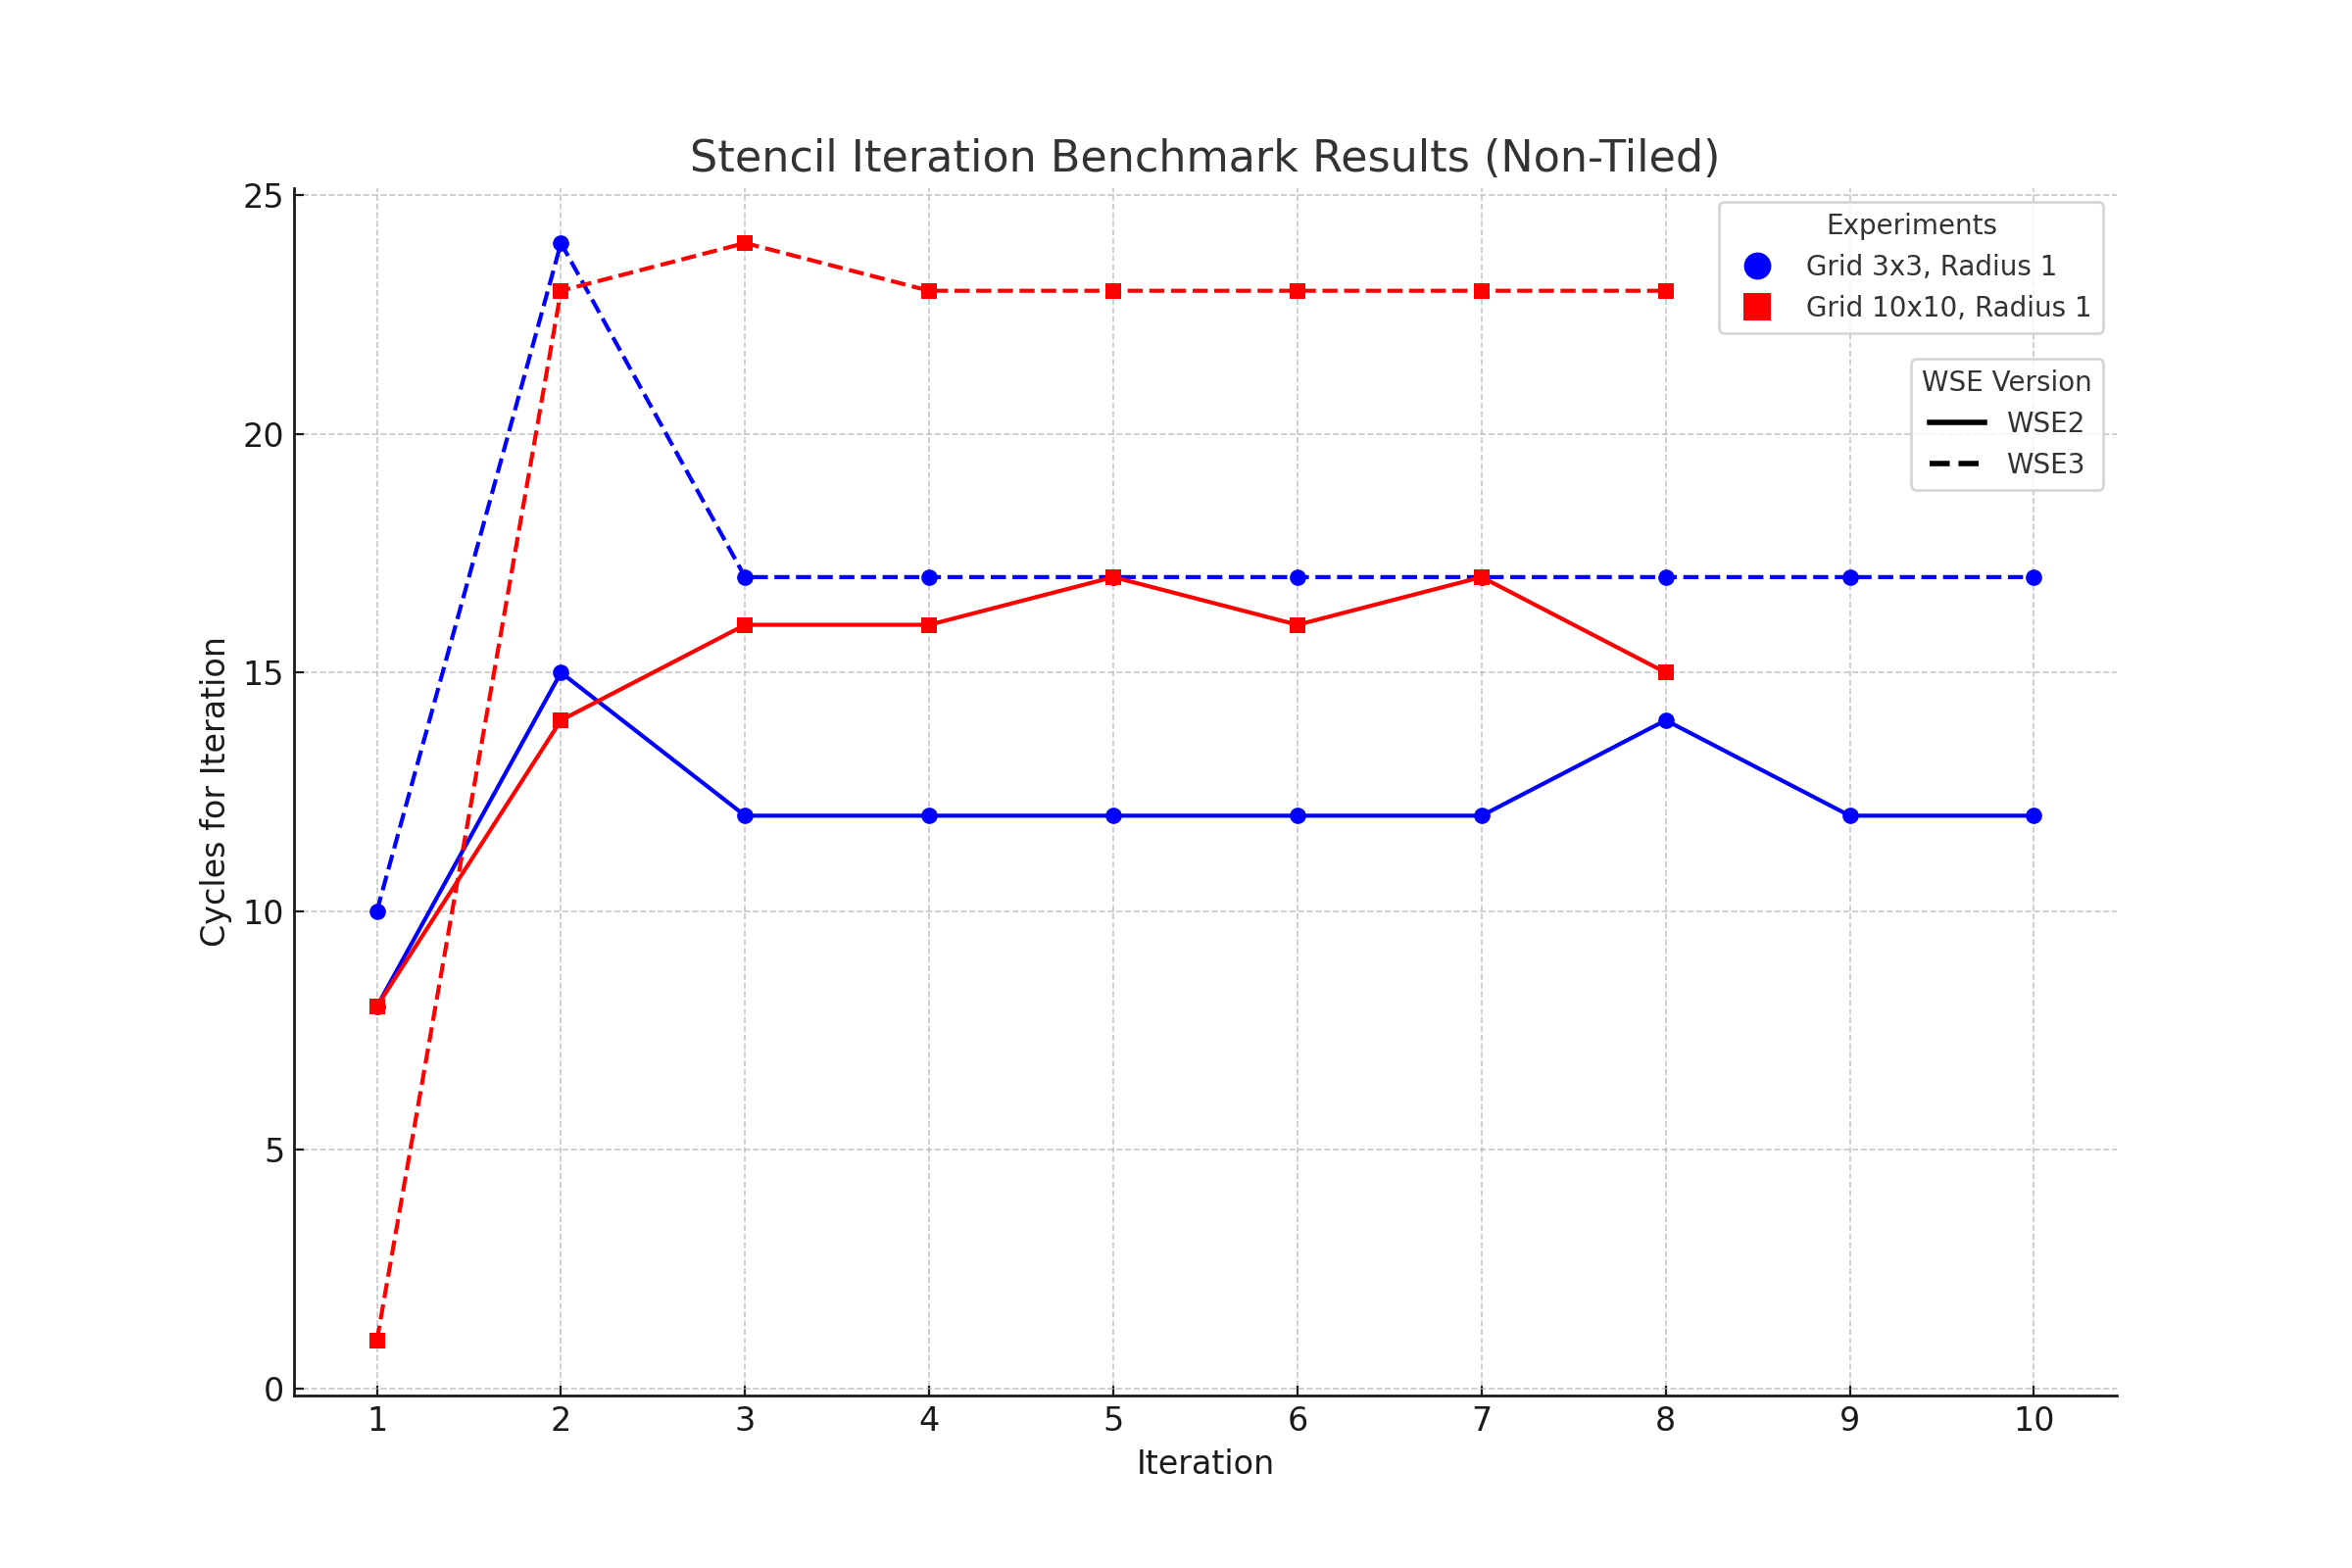
\includegraphics[width=\textwidth]{non_tiled_iteration_stability.png}
        \caption{Non-tiled algorithm}
        \label{fig:non_tiled_iteration_stability}
    \end{subfigure}
    \hfill
    \begin{subfigure}[b]{0.48\textwidth}
        \centering
        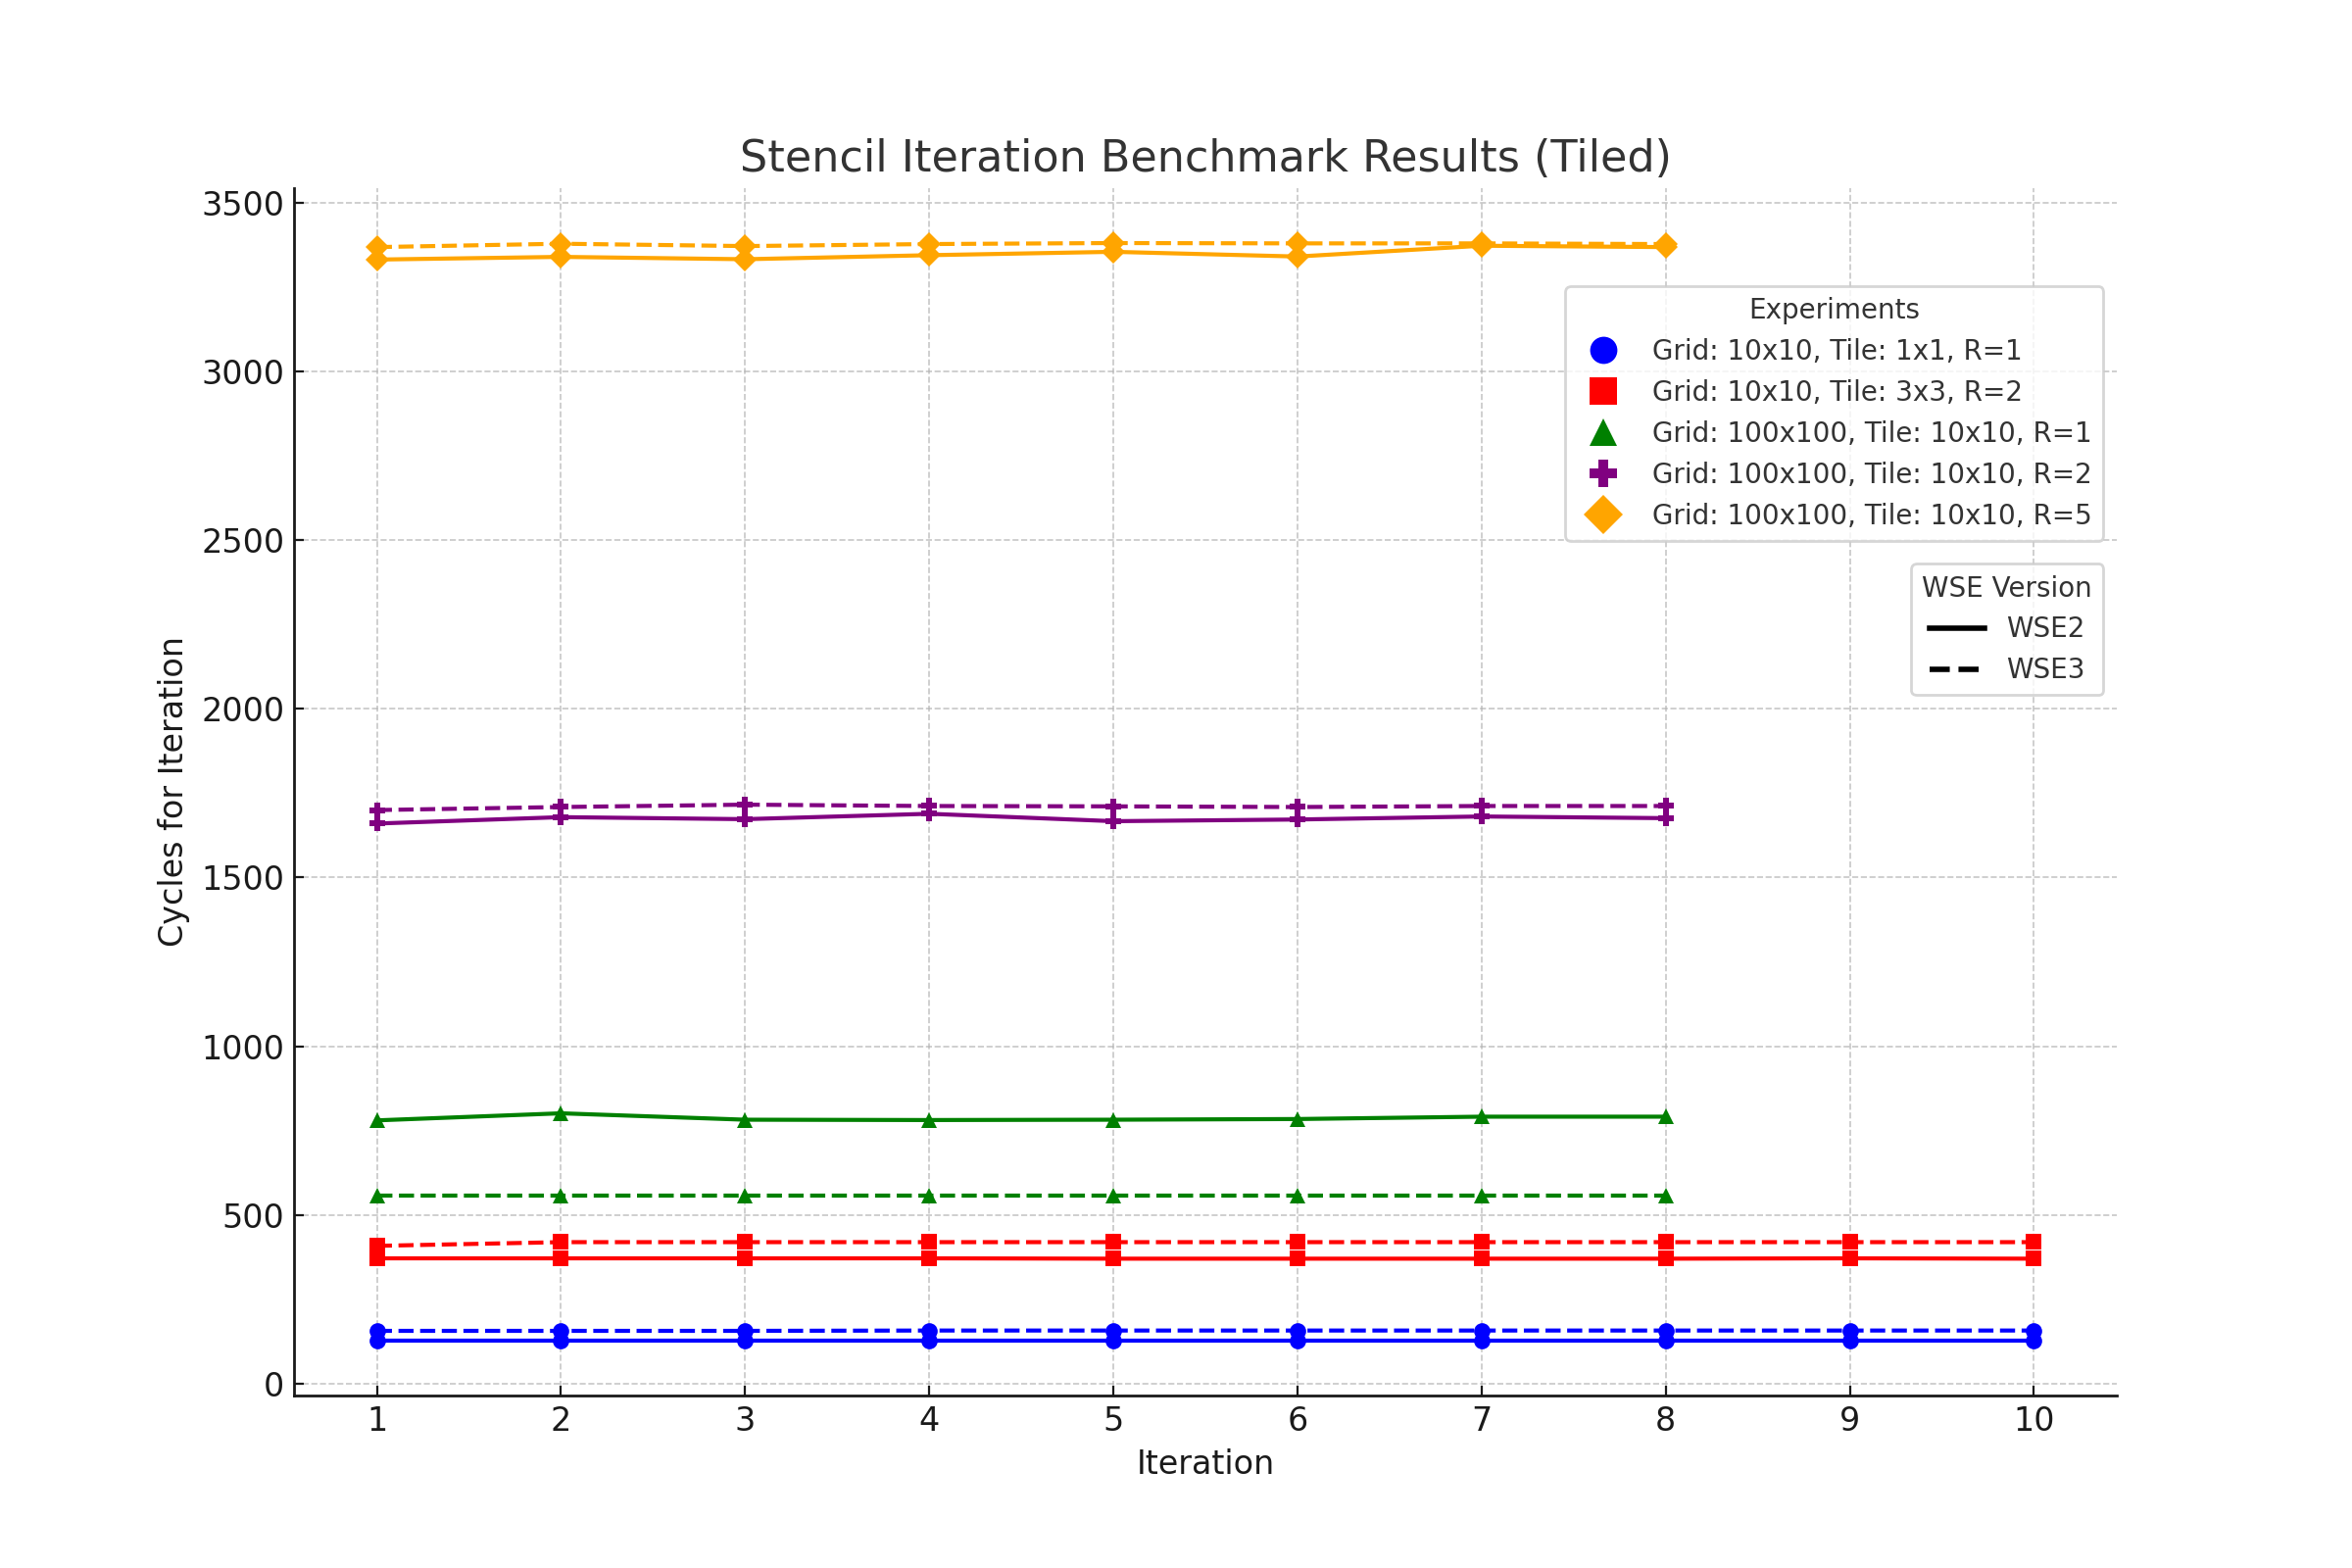
\includegraphics[width=\textwidth]{tiled_iteration_stability.png}
        \caption{Tiled algorithm}
        \label{fig:tiled_iteration_stability}
    \end{subfigure}
    \caption{Cycle count per iteration for non-tiled and tiled algorithm}
    \label{fig:iteration_stability}
\end{figure}



\section{Overhead for more \acp{pe}}
\label{sec:pe_overhead}
A very interesting question is how the performance scales with the number of \acp{pe}.
As each \ac{pe} is independent from the others, the time per iteration should be independent from the number of \acp{pe}.
This can be confirmed by the tests on the simulator up to a \ac{pe} count of \num{2500} (\numproduct{50 x 50}) for the non-tiled algorithm and \num{625} (\numproduct{25 x 25}) for the tiled algorithm.

\begin{figure}[h]
    \centering
    \begin{subfigure}[b]{0.48\textwidth}
        \centering
        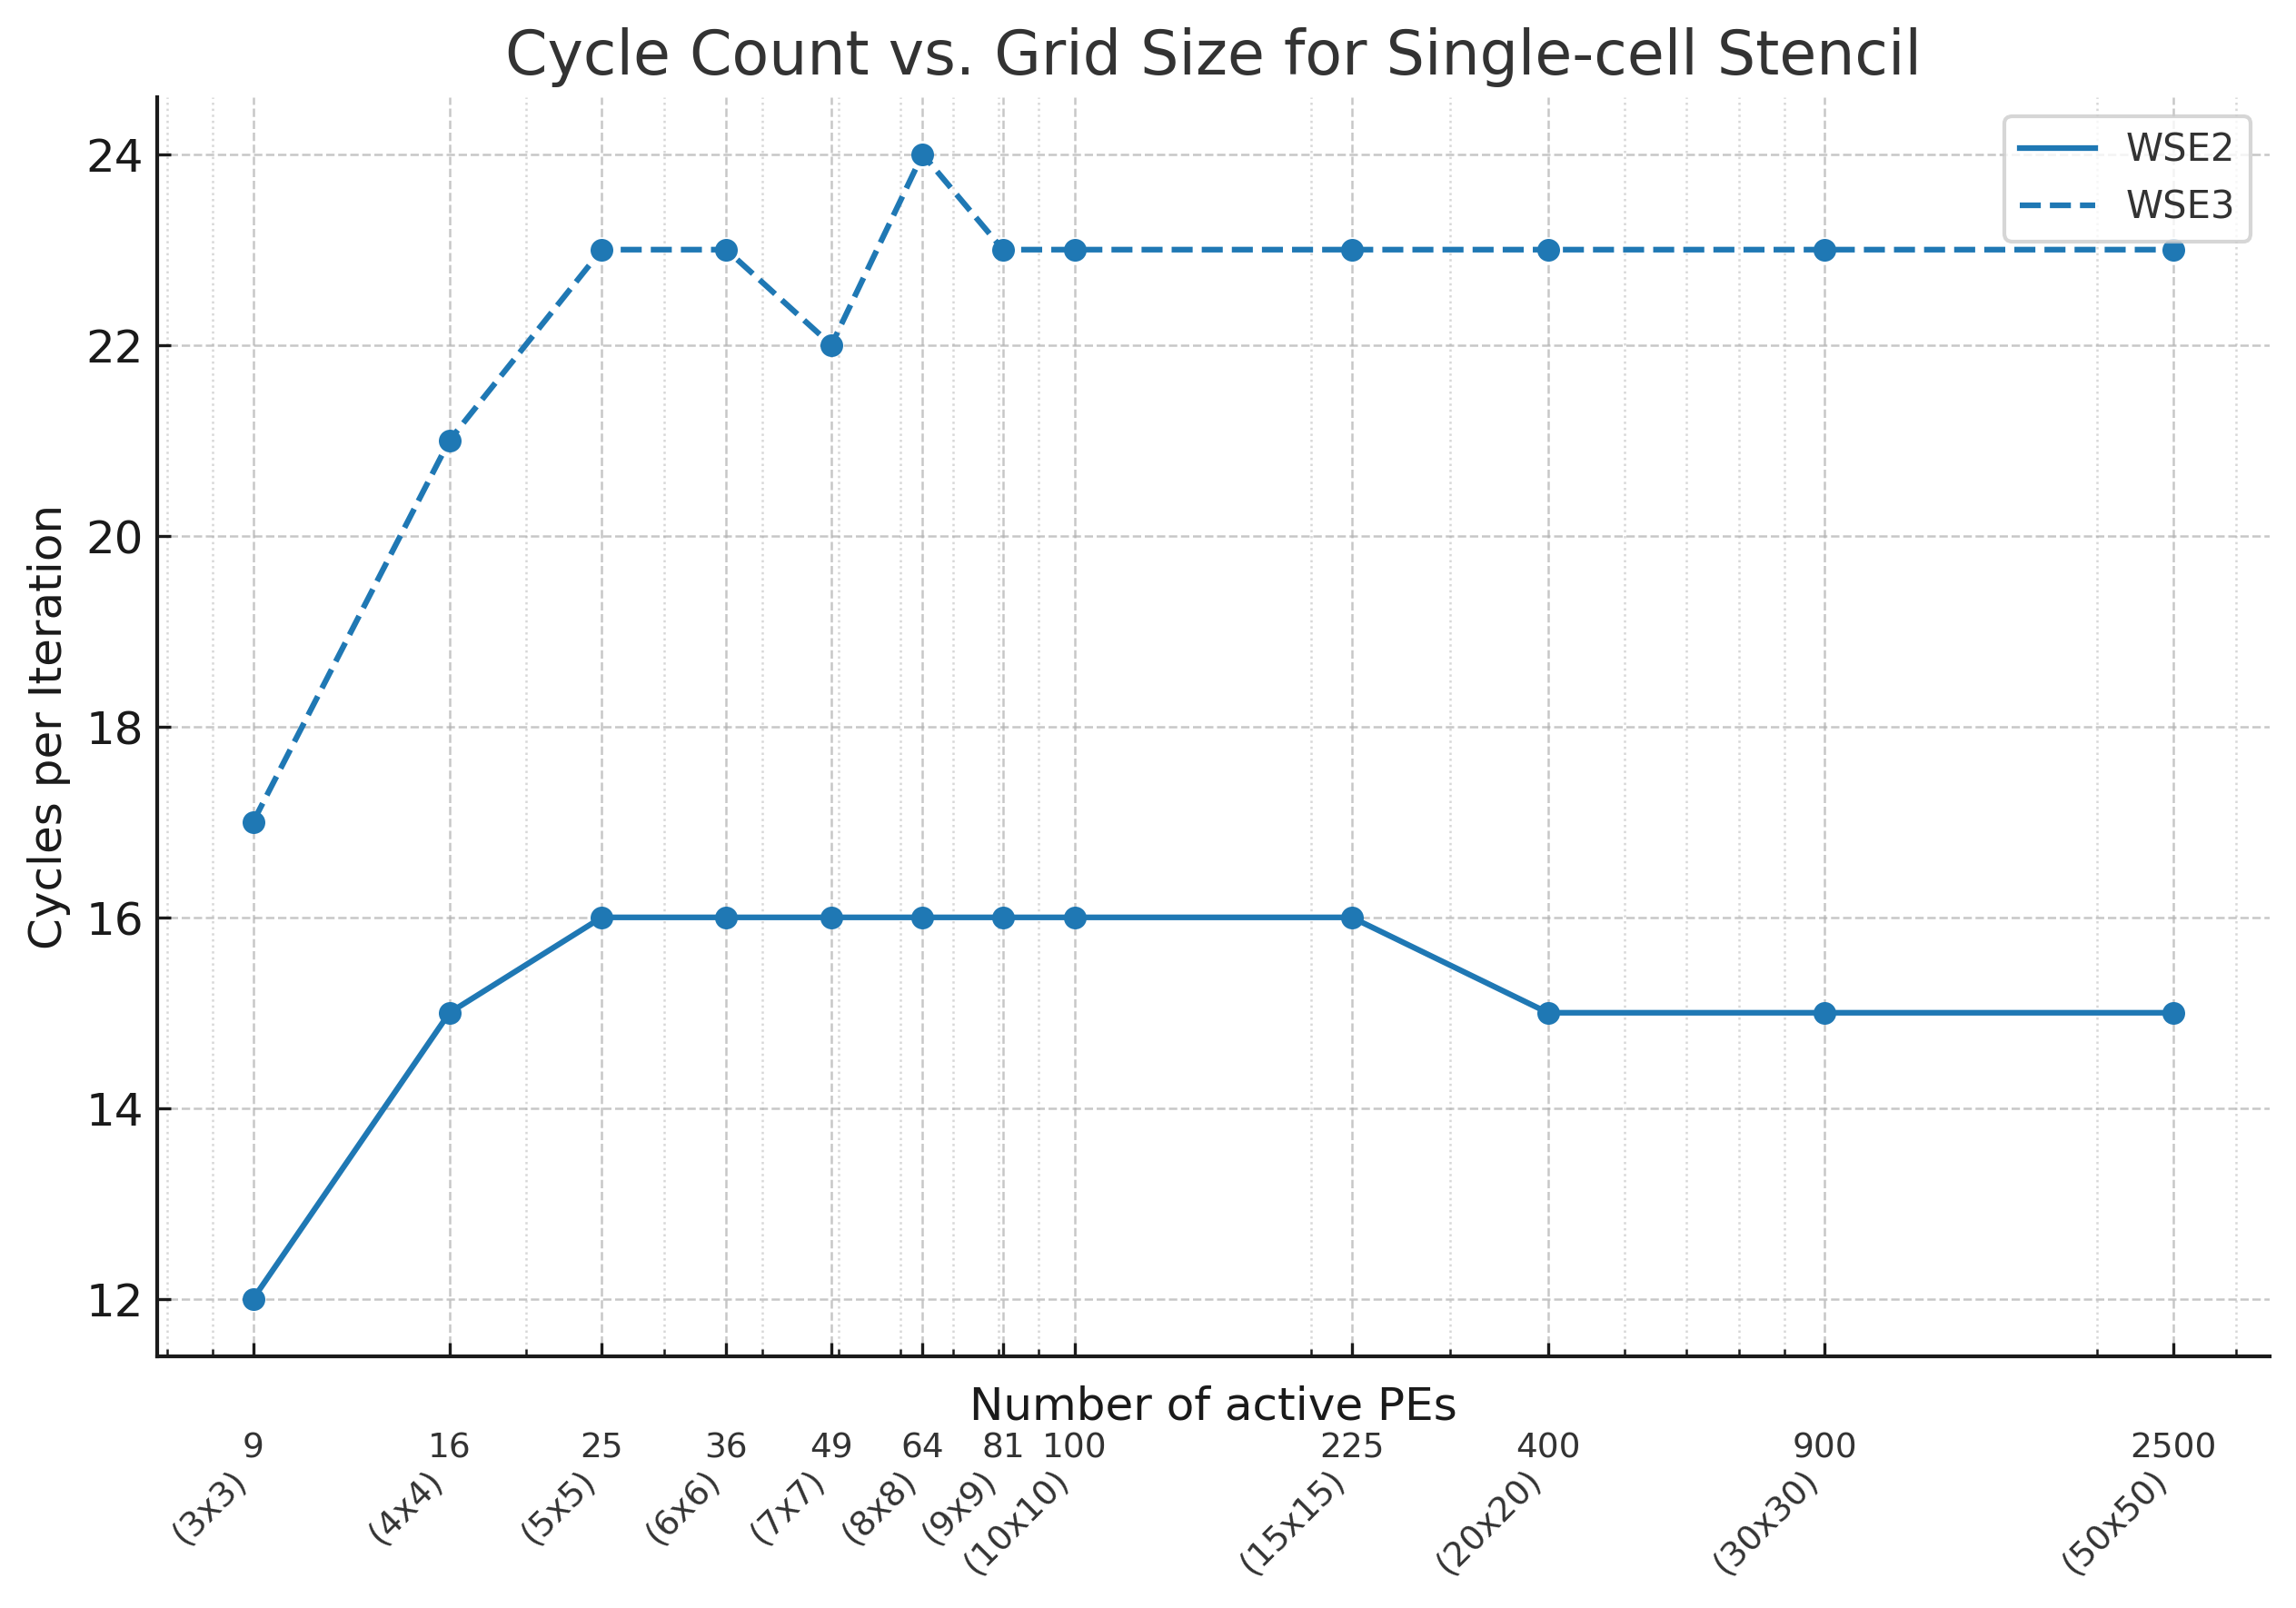
\includegraphics[width=\textwidth]{pe_overhead_non_tiled.png}
        \caption{Non-tiled algorithm}
        \label{fig:pe_overhead_non_tiled}
    \end{subfigure}
    \hfill
    \begin{subfigure}[b]{0.48\textwidth}
        \centering
        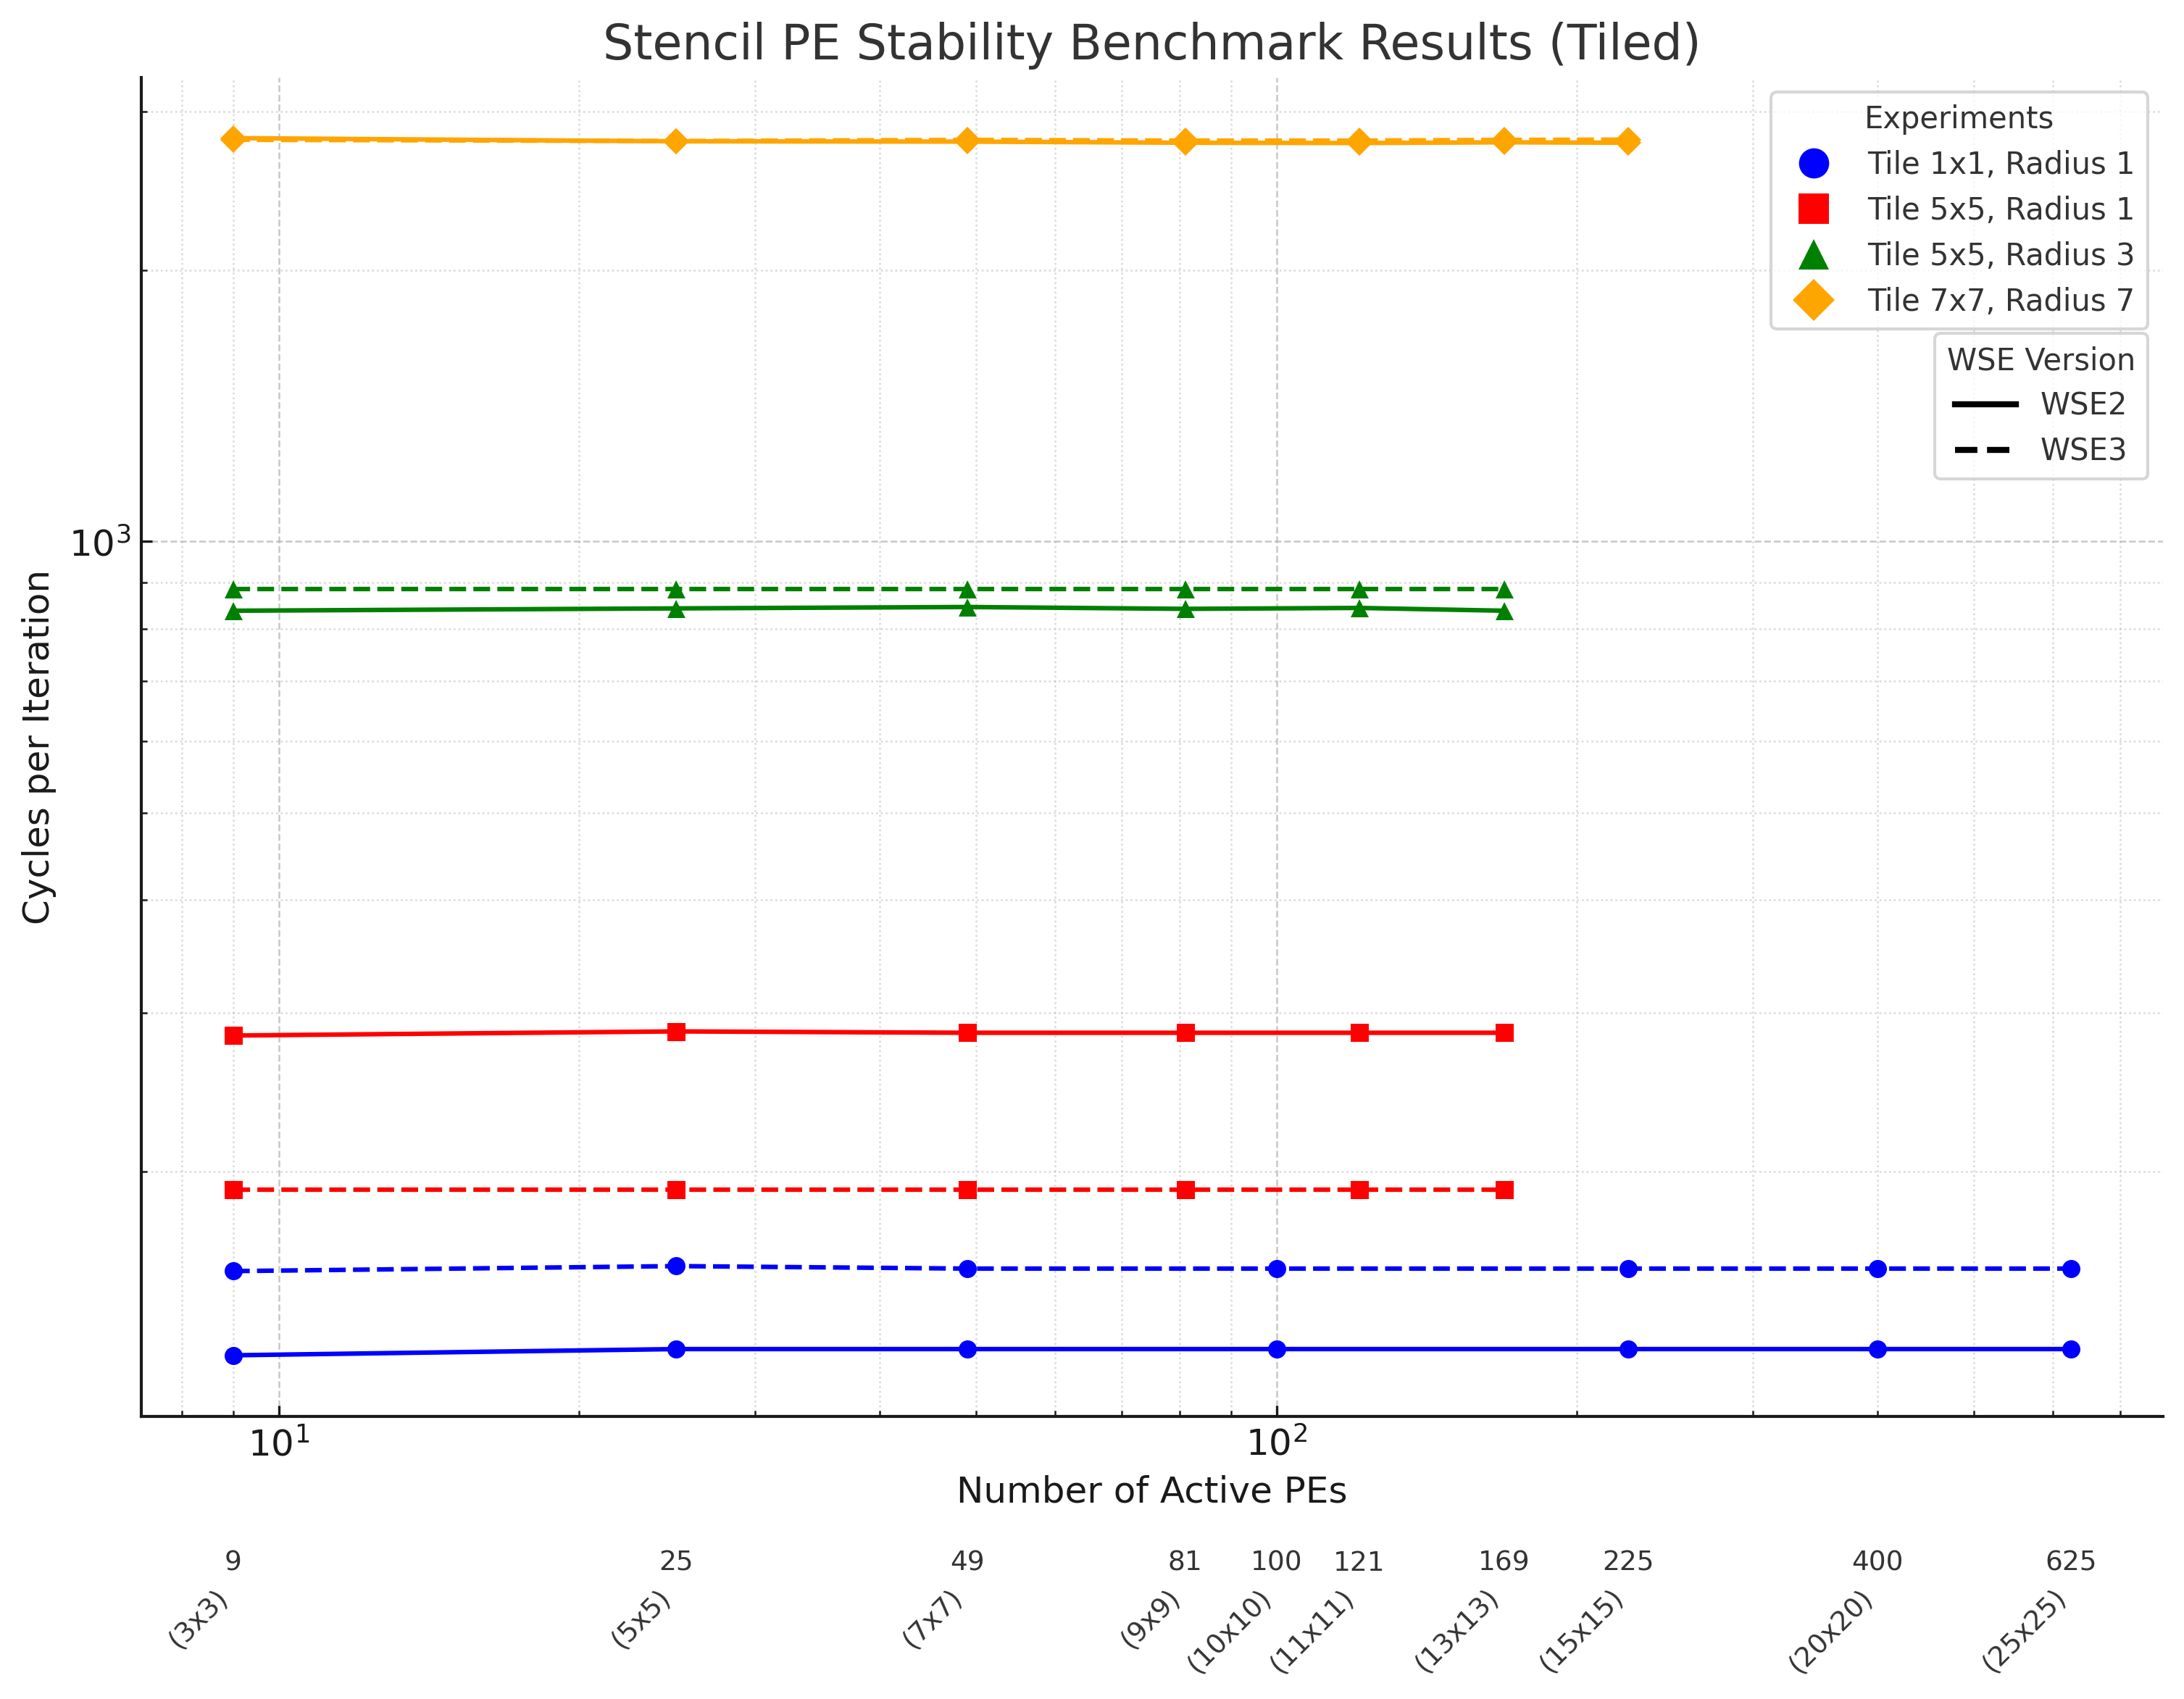
\includegraphics[width=\textwidth]{tiled_pe_stability.png}
        \caption{Tiled algorithm}
        \label{fig:tiled_pe_stability}
    \end{subfigure}
    \caption{Cycle count per iteration versus the number of active PEs for (a) the non-tiled algorithm and (b) the tiled algorithm. For the non-tiled implementation, the performance is stable for grids larger than 4x4, with the 3x3 grid showing a notably lower cycle count. The tiled implementation also demonstrates a consistent cycle count for a given configuration, independent of the number of active PEs.}
    \label{fig:pe_overhead}
\end{figure}

As shown in \autoref{fig:pe_overhead_non_tiled}, the performance of the non-tiled algorithm scales almost perfectly, with the cycle count remaining constant with minimal fluctuations regardless of the grid size. The one exception is the 3x3 grid, which is significantly faster. We hypothesize this is an artifact of the experimental setup where only the single, inner \ac{pe} is performing computation and does not need to synchronize with other computing neighbors, effectively eliminating the communication latency discussed in \autoref{sec:theoretical_performance_evaluation_and_comparison_against_roofline_model}. For all subsequent experiments, we ensure at least \numproduct{5 x 5} active \acp{pe} - which results in at least \numproduct{3 x 3} \acp{pe} inner \acp{pe} - to provide representative results.

Jacquelin et al. \cite{jacquelin2022massively} show that for a 3d stencil that is tested on real hardware, the cycle count scales almost perfectly with the number of \acp{pe} up to the whole \ac{wse} dimensions.
We therefore expect that our implementation also scales nearly perfectly on the real hardware and calculate with this assumption in the following experiments.

\section{Maximum tiling size}
The maximum tiling size that fits into the memory of a \ac{pe} is limited by the number of memory banks and the size of the data structure registers.
We test this by increasing the tile size to the maximum that still compiles for (test wse2 and wse3 independently!!! currently same number for both (smaller one))

We find that the maximum tiling size  is 64x64=4096 elements.
A non-quadratical tile size, that results in 4096 elements, is likely also possible, but not tested.
Tile size of 64x64 was tested up to radius 3. It is likely to decrease for larger radius.

This results in a maximum grid size containing \num{3101280000} elements on wse-2 and \num{3670474752} elements on wse-3.
Note that due to hardware limitations of the \ac{wse}, the maximum stride for \acp{dsd} is \num{127} which makes very uneven distributions between tile width and tile height not possible.


\section{Comparison of non-tiled and tiled algorithm}

The non-tiled algorithm is implemented in a completely different way than the tiled algorithm.
This allows for a very optimized implementation, that doesn't require any runtime \ac{dsd} to \ac{dsr} transfers, asynchronous operations and task activation.
It is therefore significantly faster than the tiled algorithm for radius 1.
However, the non-tiled algorithm is naturally limited to a radius of 1 and a grid size not larger than the \ac{wse} dimensions.

\begin{figure}[h]
    \centering
    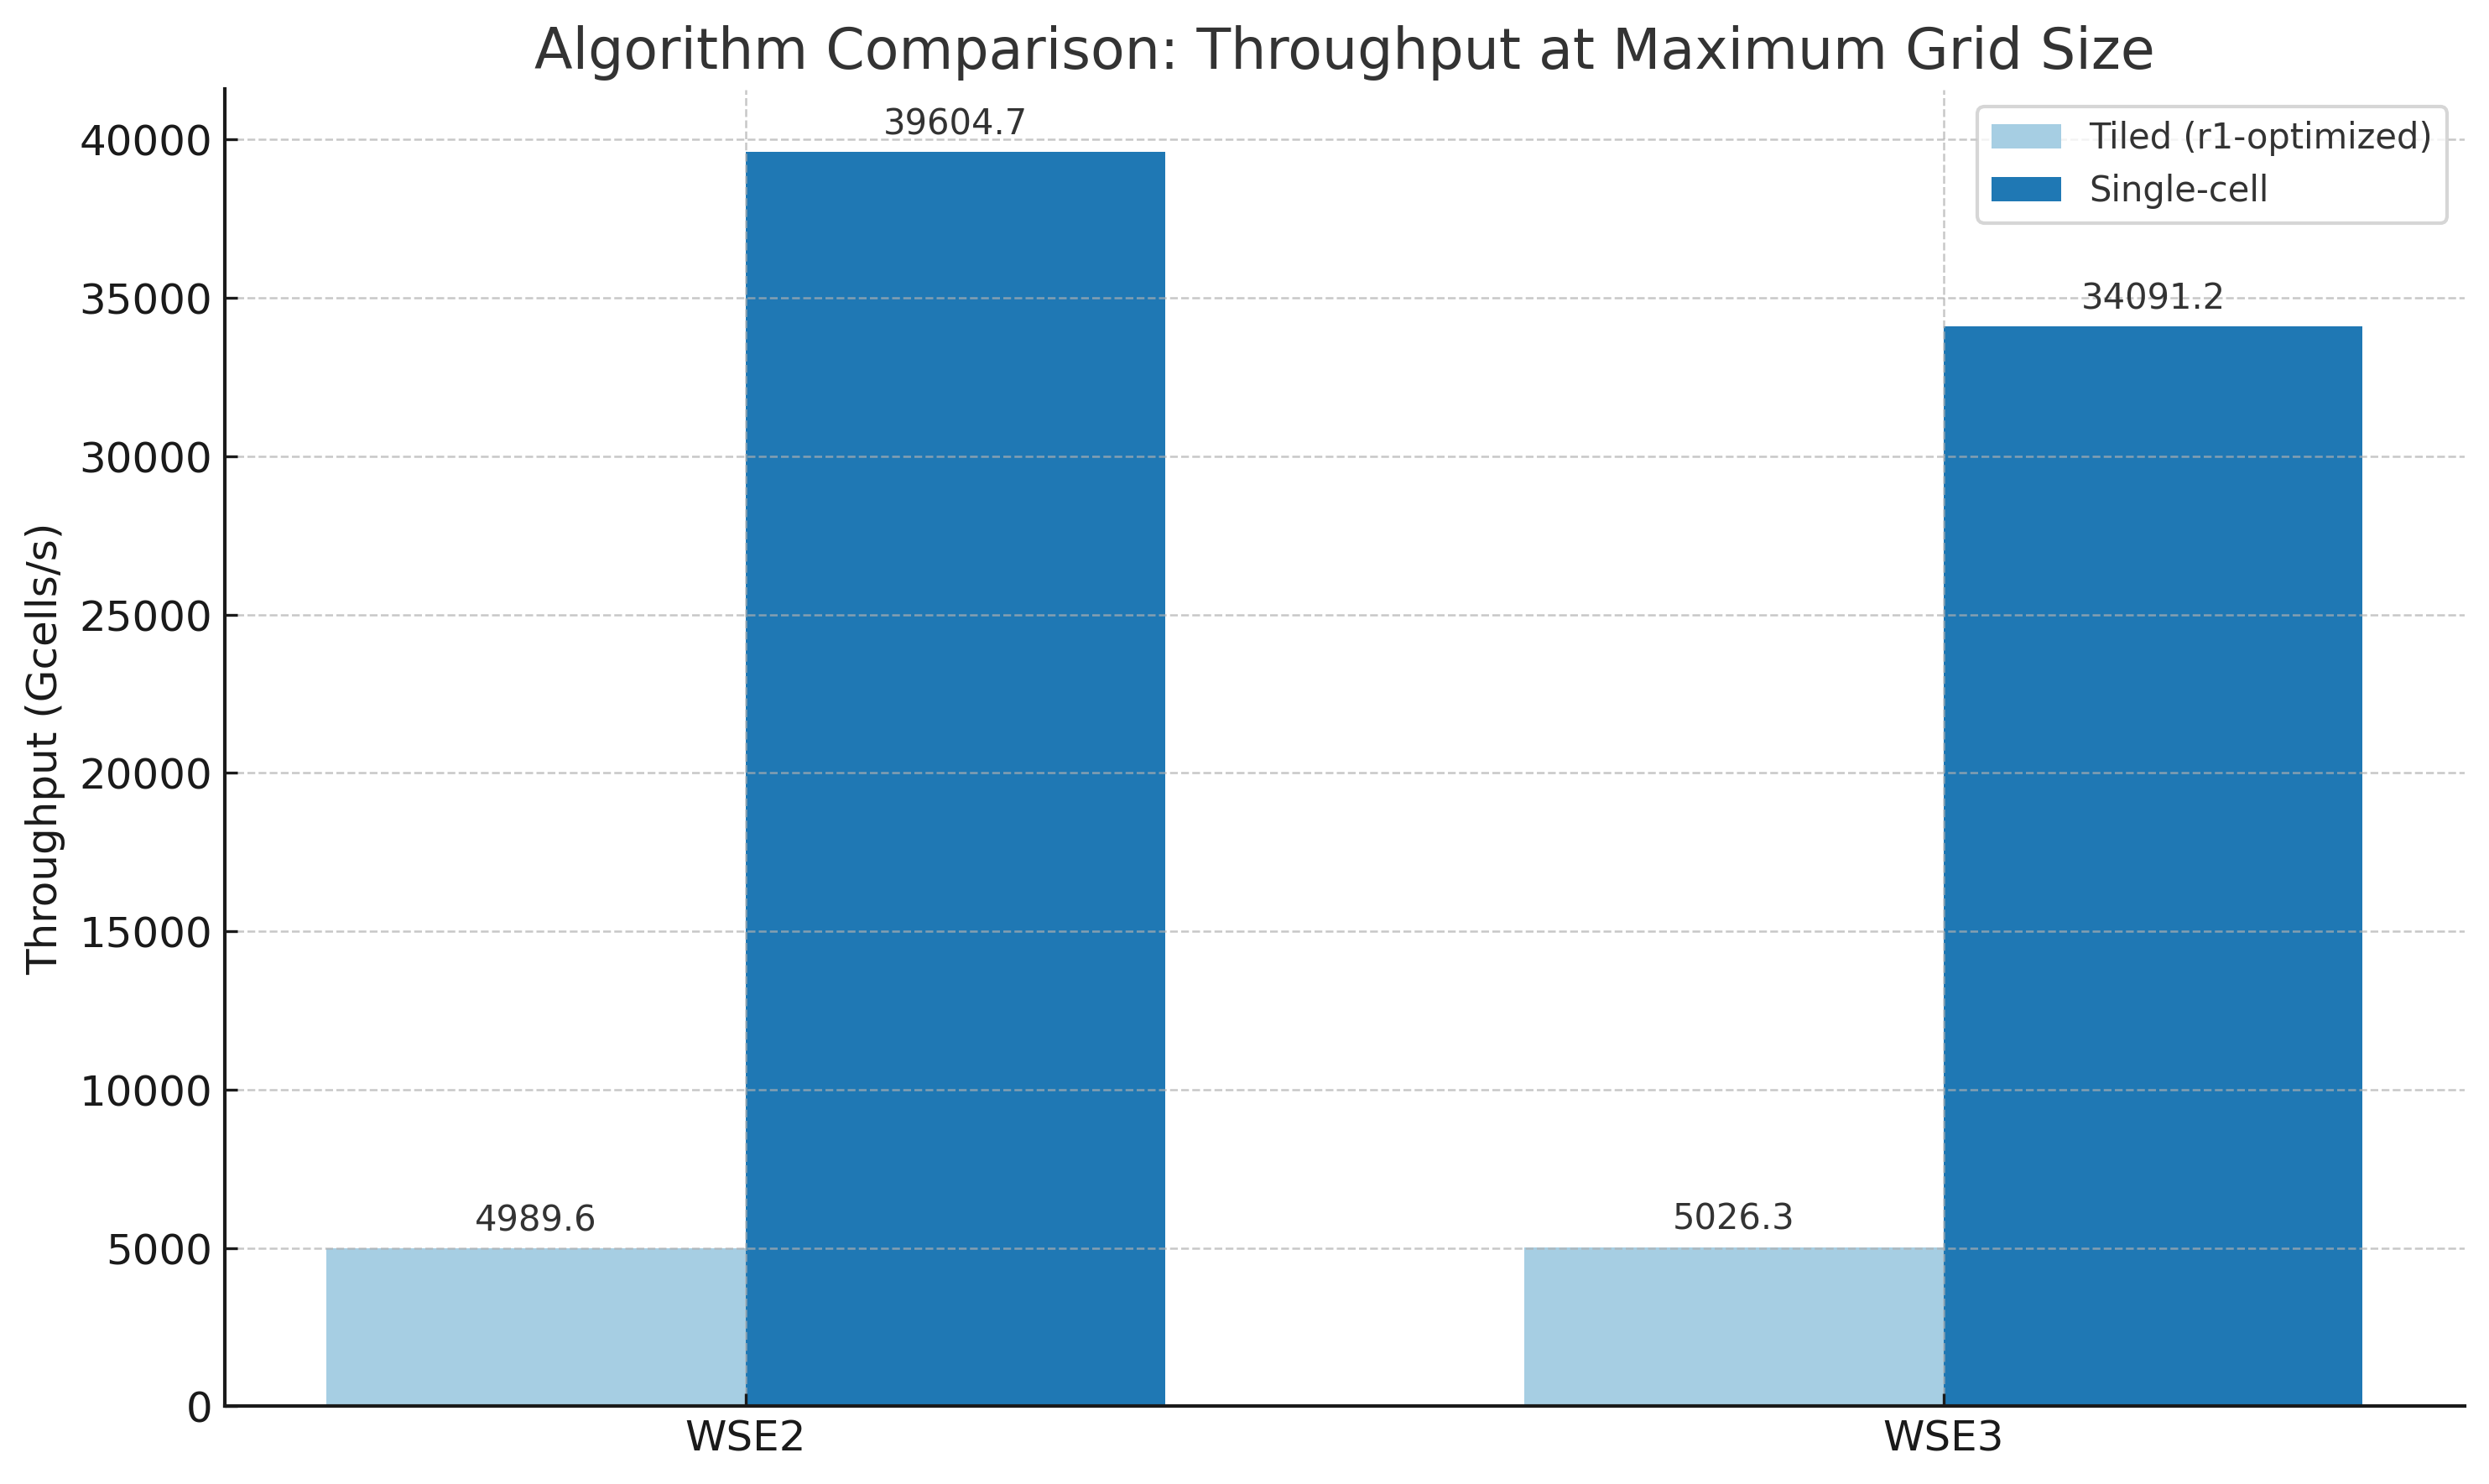
\includegraphics[width=0.5\linewidth]{algo_comparison.png}
    \caption{Performance comparison of the specialized non-tiled and the r1-optimized tiled implementations for a radius-1 stencil. The specialized, non-tiled algorithm is significantly faster, achieving an 8x speedup on \ac{wse}-2 and a 7x speedup on \ac{wse}-3 due to its simpler communication and execution model.}
    \label{fig:algo_comparison}
\end{figure}

\section{Comparison of Cerebras and traditional \ac{hpc}-Arcitectures}
We conducted two more experiments to compare the performance of the implemented stencil on the Cerebras \ac{wse} with highly optimized Devito implementations for \ac{cpu} and \ac{gpu}. The experiments were conducted using the Vast.ai cloud.
For the \ac{cpu} experiments we used a system with two AMD EPYC 9554 64-Core processors. The system has a total of \qty{128}{\mega\byte} of L2 cache and \qty{512}{\mega\byte} of L3 cache. It is equipped with \qty{1511}{\giga\byte} of DDR5 memory.
The system is furthermore equipped with a NVIDIA H100 SXM 80GB, which was used for the \ac{gpu} experiments. The system had CUDA 12.8 installed and we used python 3.12.11, Devito 4.8.19, Cupy 13.4.1 and the nvc compiler in version 25.5.

For each benchmark we fixed the total work load, i.e., $width\times height\times N$, so that every configuration performs the same number of stencil updates while varying only the memory footprint. Steady-state performance was obtained by first running an untimed warm-up of $N$ iterations (triggering JIT compilation, allocations and data transfers) and then timing a second run of the same $N$ iterations with all data already resident on the \ac{cpu} or \ac{gpu}. This was done for grids with a total size of $10^x$ for $x \in \{4..9\}$ and radii in \numrange{1}{6}.
The compute work, while in this experiment constant for different grid sizes, rises linearly with the radius, which on the other hand has no significant effect on memory footprint.
Furthermore, we calculated the neccessary tile size to fit the same grid sizes on the \ac{wse}-3 and ran an experiment with this tile size for radii \numrange{1}{6} and a total grid size that results in \numproduct{5 x 5} active \acp{pe} in the simulator for four iterations and took the average cycle count of the last two iterations.
Assuming perfect scaling accross the WSE as suggested by the results from \autoref{sec:pe_overhead}, we used this cycle count together with the \ac{wse}s clock frequency to calculate the total time for $10^{10-x}$ iterations.
We also added the time, the non-tiled algorithm would take on the \ac{wse}-3 for the respective number of iterations where the \ac{wse}-3s hardware dimensions allow for the grid size.
As the $width$ and $height$, we strictly used powers of 10, resulting in rectangular grids for odd $x$.
To have all experiments use \numproduct{5 x 5} active \acp{pe} in the simulator, we used a grid size of $\roundbrack{3\times t_w + 2r, 3\times t_h + 2r}$.

To ensure the entire problem grid fits onto the available \acp{pe} of the \ac{wse}, the tile size ($t_w$, $t_h$) for a given grid of size ($G_w$, $G_h$) on a \ac{wse} with physical dimensions ($P_w$, $P_h$) is determined by:
\begin{equation}
    t_w = \left\lceil \frac{P_w}{G_w} \right\rceil, \quad t_h = \left\lceil \frac{P_h}{G_h} \right\rceil
\end{equation}

For example, to map the \numproduct{10e3 x 10e4} grid onto the \ac{wse}-3 with its \numproduct{762 x 1176} \acp{pe} array, we calculate the tile size. Mapping the grid's width to the \acp{pe} array's width results in a tile width of $\left\lceil \frac{1000}{762} \right\rceil = 2$ and a tile height of $\left\lceil \frac{10000}{1176} \right\rceil = 9$. However, mapping the grid's width to the \acp{pe} array's height is more efficient, yielding a tile width of $\left\lceil \frac{1000}{1176} \right\rceil = 1$ and a tile height of $\left\lceil \frac{10000}{762} \right\rceil = 14$. To minimize the total tile area and therefore the per-\ac{pe} workload, we chose the smaller configuration of $1 \times 14$. It is important to note that due to the radius constraint from \autoref{eq:radius_constraint}, the shorter dimension of the tile must be at least as large as the radius, so the effective tile size was adjusted accordingly if necessary.

\begin{table}[h]
    \centering
    \caption{Final parameters for the experiment in the simulator for a grid size of \num{1e7}}
    \begin{tabular}{ll}
        \hline
        Parameter & Value \\
        \hline
        Grid size & \numproduct{5 x 44} \\
        Tile size & \numproduct{1 x 14} \\
        Radius & \num{1} \\
        Number of iterations & \num{2} and \num{4} \\
        \hline
    \end{tabular}
    \label{tab:sim_params}
\end{table}

\begin{figure}[h]
    \centering
    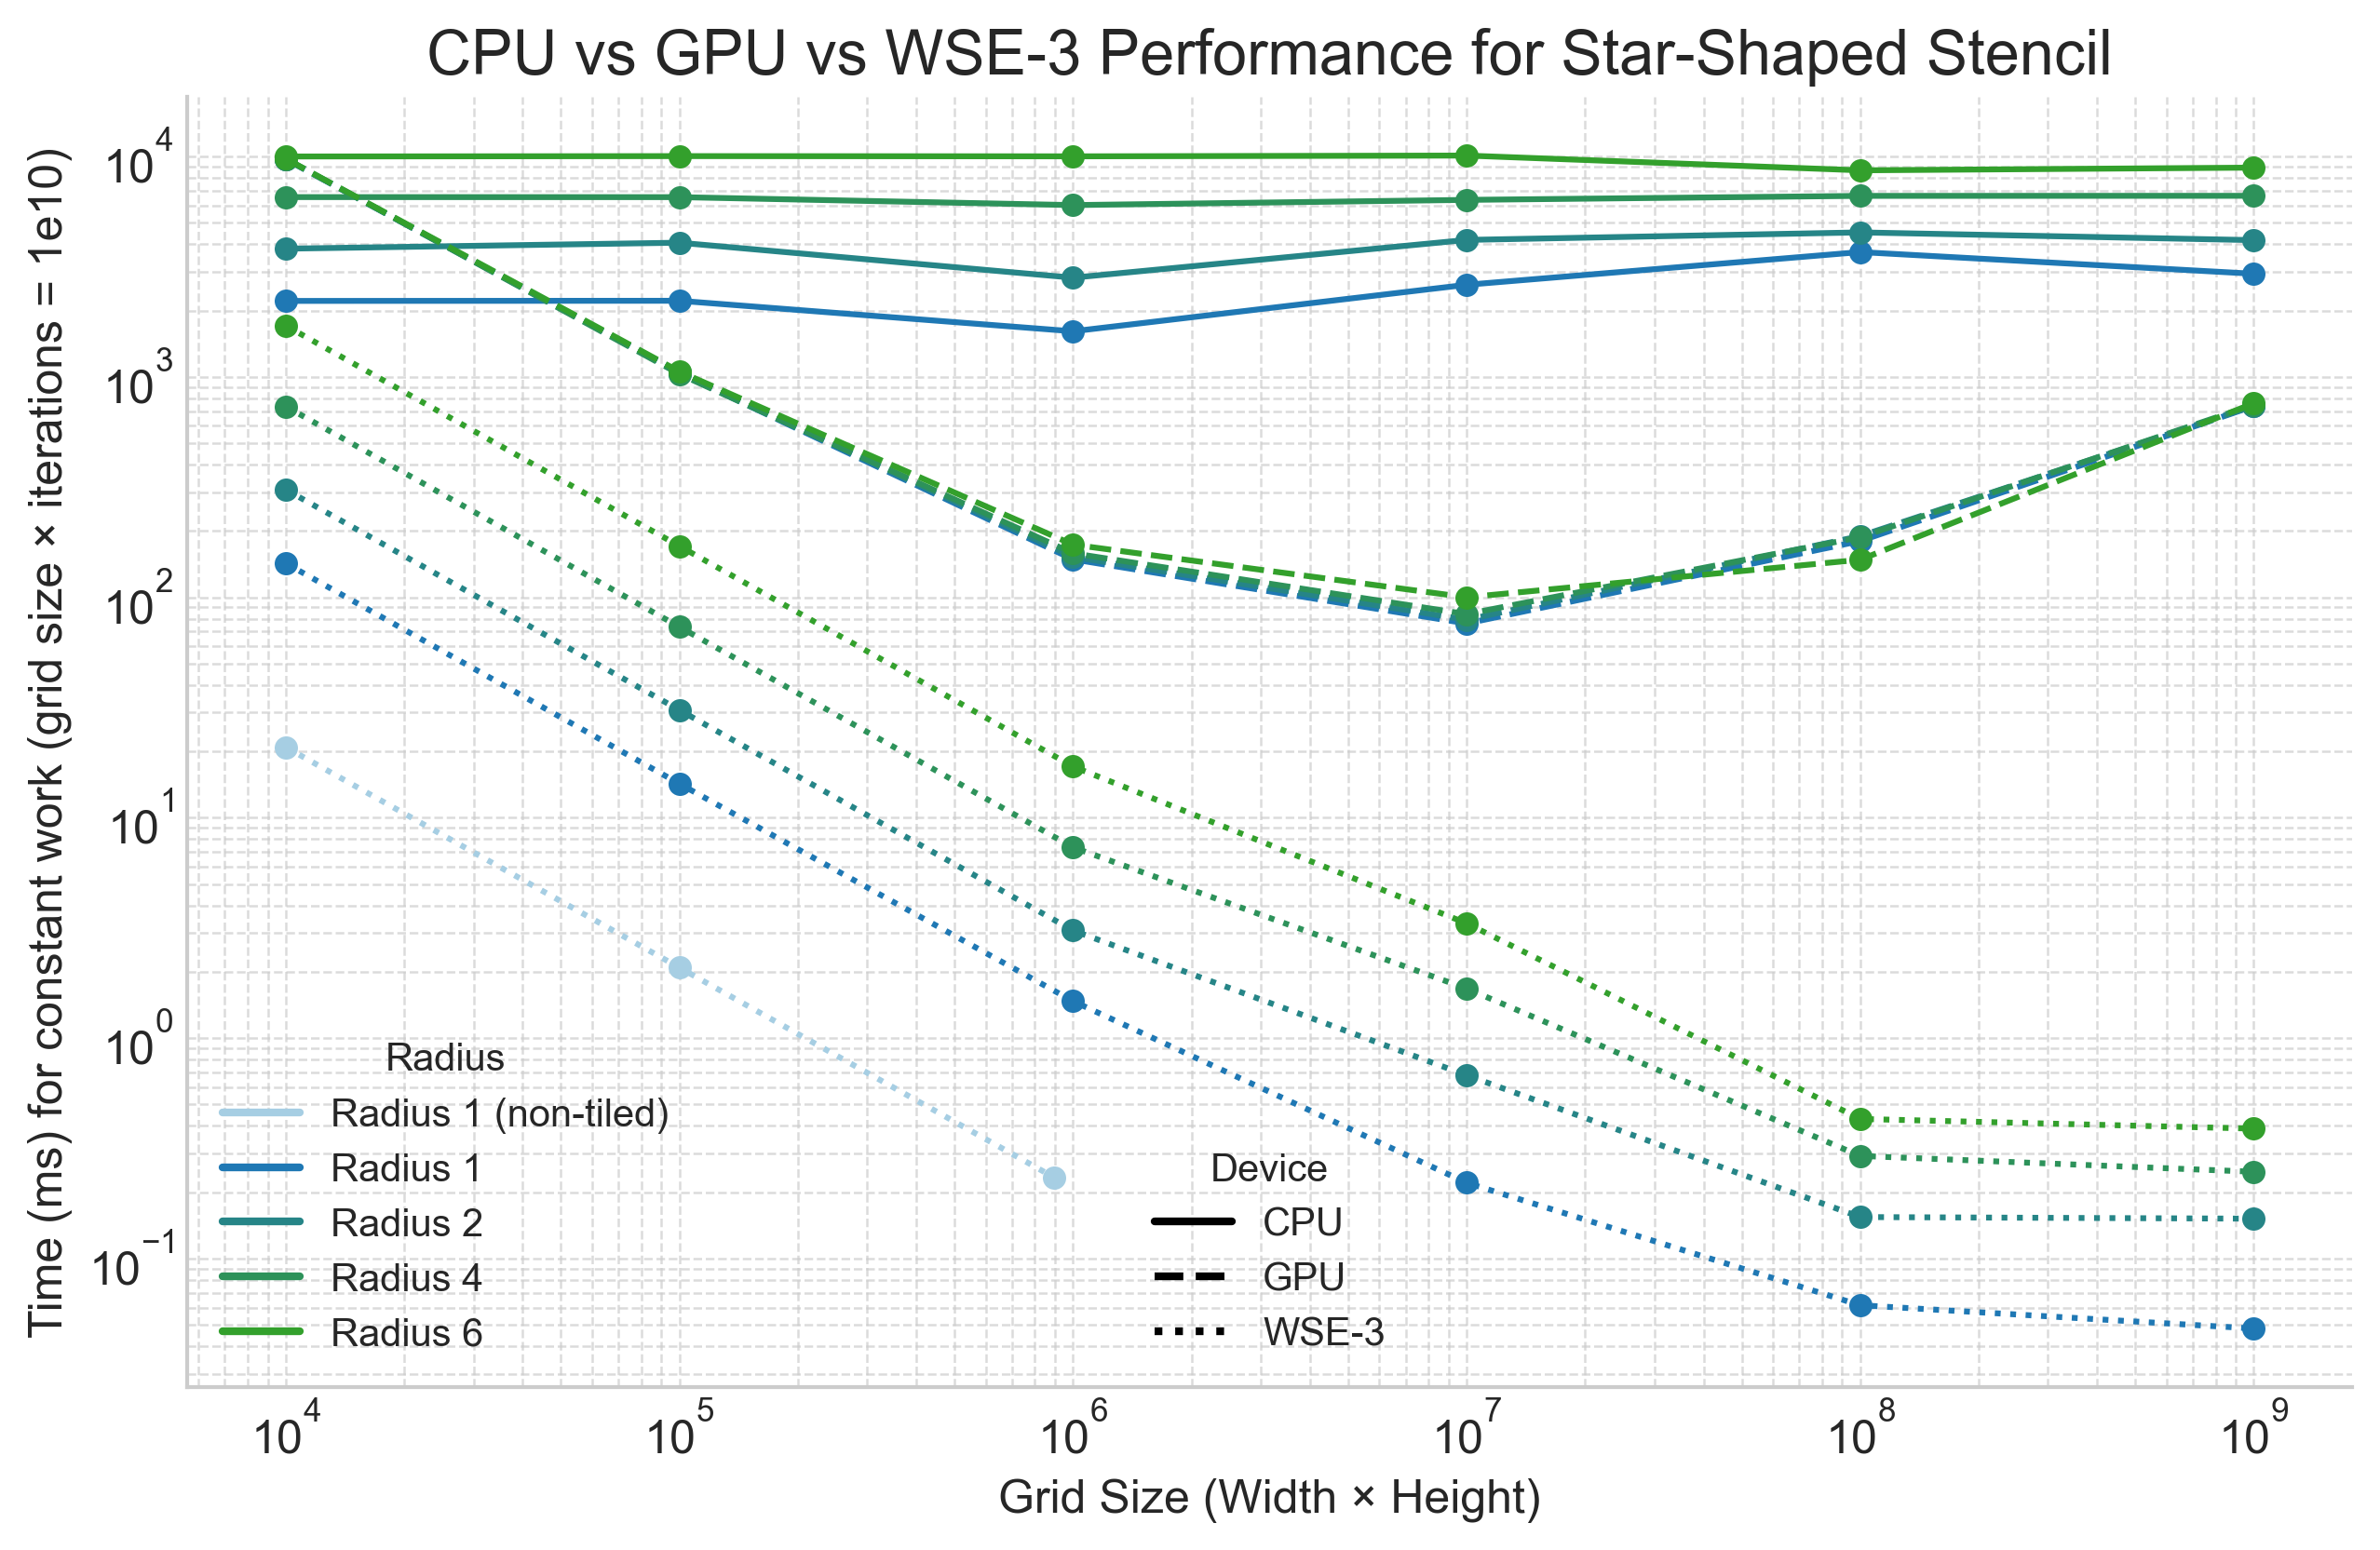
\includegraphics[width=1\linewidth]{gpu_cpu_wse3_constant_product.png}
    \caption{Comparison of \ac{cpu} and \ac{gpu} performance for different grid sizes and number of iterations, so that $width \times height \times iterations = \num{1e10}$}
    \label{fig:gpu_cpu_constant_product}
\end{figure}

The results, shown in \autoref{fig:gpu_cpu_constant_product}, show that the \ac{cpu} is very insensitive to the work allocation and differs only by a factor of \num{2.3} between its ideal grid size of \num{1e6} its least ideal grid size of \num{1e8} at a radius of 1. For the largest tested radius of \num{6} this effect is even smaller at a factor of \num{1.2} between fastest and slowest run.

The \ac{cpu}s insensitivity to the work allocation suggests that it is compute limited.
This gets confirmed by the fact that the \ac{cpu} runtime scales almost linearly with the radius. For the \ac{cpu} and its optimal grid size of $\num{1e6}$, it takes \num{6.2} times longer to calculate the \num{6} times as computationally expensive radius-\num{6} stencil compared to the radius-\num{1} stencil.

Furthermore we observe that \ac{gpu} performance differs significantly depending work allocation with a minimal time of \qty{7.6e-2}{\second} for the optimal grid size of $\num{1e7}$ and a 128x slower time of \qty{9.7}{\second} for the slowest grid size of $\num{1e4}$. Interstingly a very large grid size of $\num{1e9}$ at a time of of \qty{7.4e-1}{\second} also results in a 9.7x slower time than the optimal grid size. While looking for a possible explanation for the pronounces optimum at a grid size of \num{1e7}, we find that the required memory of $\num{1e7}\times\qty{4}{\byte}=\qty{40}{\mega\byte}$ fits perfectly into \qty{50}{\mega\byte} L2 cache of the H100.
Other than the \ac{cpu}, the \ac{gpu} is very insensitive to the radius. So much that all differences in the runtime for different radii are more likely attributed to measurement errors than to a real difference in the runtime.
This strongly suggests that the \ac{gpu} is memory limited through all the different tested grid sizes.

The results show that for most tested configurations, the \ac{gpu} outperforms the \ac{cpu}.
However for very small tile sizes of \numproduct{100 x 100} and large iteration counts of $\num{1e6}$, the \ac{cpu} is faster.

The \ac{wse}-3 is very sensitive to both the work allocation and the radius. The sensitivity to radius is significant accross all grid sizes with a factor of \num{12.0} between radius \num{1} and \num{6} for a grid of \num{1e4} and factor of \num{8.1} between radius \num{1} and \num{6} for a grid of \num{1e9}.
The more than linear scaling for small grid sizes can be explained by the fact that these problems use a tile size of \numproduct{1 x 1} for radius \num{1} and \numproduct{6 x 6} for radius \num{6} which results in $r^2(10r-1)$ flops per \ac{pe}. This number rises with the cube of $r$. The 12x now appears relatively low and is caused by communication also playing a major role in the overall time for these small grid sizes. For a grid size of \num{1e9} on the other hand, the tile size is constant for all radii and the scaling is closer to linear with an outlier for radius \num{1}, because this uses the $r1$ optimized tiled algorithm. The factor between radius \num{2} and \num{6} is \num{2.6}.

Analyzing the \ac{wse}-3s performance, we find that the iterations per second (not shown in the plot!) is constant for grids of size \numrange{1e4}{1e6}. Together with the decreased number of iterations for larger grid sizes, this leads to faster runtimes for larger grid sizes. This is because grid sizes smaller than \num{1e6} do not use the whole \ac{wse} dimensions and the scaling to more \acp{pe} comes without performance degradation. Grid sizes from \num{1e6} to \num{1e8} use the whole \ac{wse} and show slower iteration times as the grid size increases, but sublinear. For radius \num{1} the slowdown of time per iteration between grid sizes of \num{1e6} and \num{1e7} is only \num{1.5} and from \num{1e7} to \num{1e8} only \num{2.8}. However starting from \num{1e8} the slowdown is almost linear with a factor of \num{7.8} between \num{1e8} and \num{1e9} for radius \num{1} and \num{9.8} for radius \num{2}. We assume this is because constant overheads are getting less significant relative to the computation at these grid sizes.

The \ac{wse}-3 implementation outperforms the \ac{cpu} and \ac{gpu} for all tested grid sizes and radii with the most significant speedup for the largest grid size of \num{1e9} and radius \num{1} with a speedup of \num{1.5e4} compared to the \ac{gpu} and \num{6.1e4} compared to the \ac{cpu}. Because the runtime for the stencil is independent from the radius on the \ac{gpu}, but not on the \ac{wse}-3, the speedup from \ac{wse}-3 to \ac{gpu} for the same grid size of \num{1e9} and radius \num{6} is significantly smaller at \num{2.0e3}.


% As a second experiment, we compared our implementation for a grid size of the \ac{gpu}-optimal $\num{1e7}$ to the optimized \ac{gpu} and \ac{cpu} implementation. To fit a size of $\num{1e3}\times\num{1e4}$ on the \ac{wse}-2 with dimensions of $750\times994$, we need a tile size of at least $2x11$ and on \ac{wse}-3 with dimensions of $762\times1176$ a tile size of at least $14x1$. As shown in the earlier experiments, degrade larger tile sizes always the performance so we used these minimum tile sizes. Because of the radius constraint from \autoref{eq:radius_constraint}, we need to increase the shorter dimension of the tile to the respective radius.

% \begin{figure}[h]
%     \centering
%     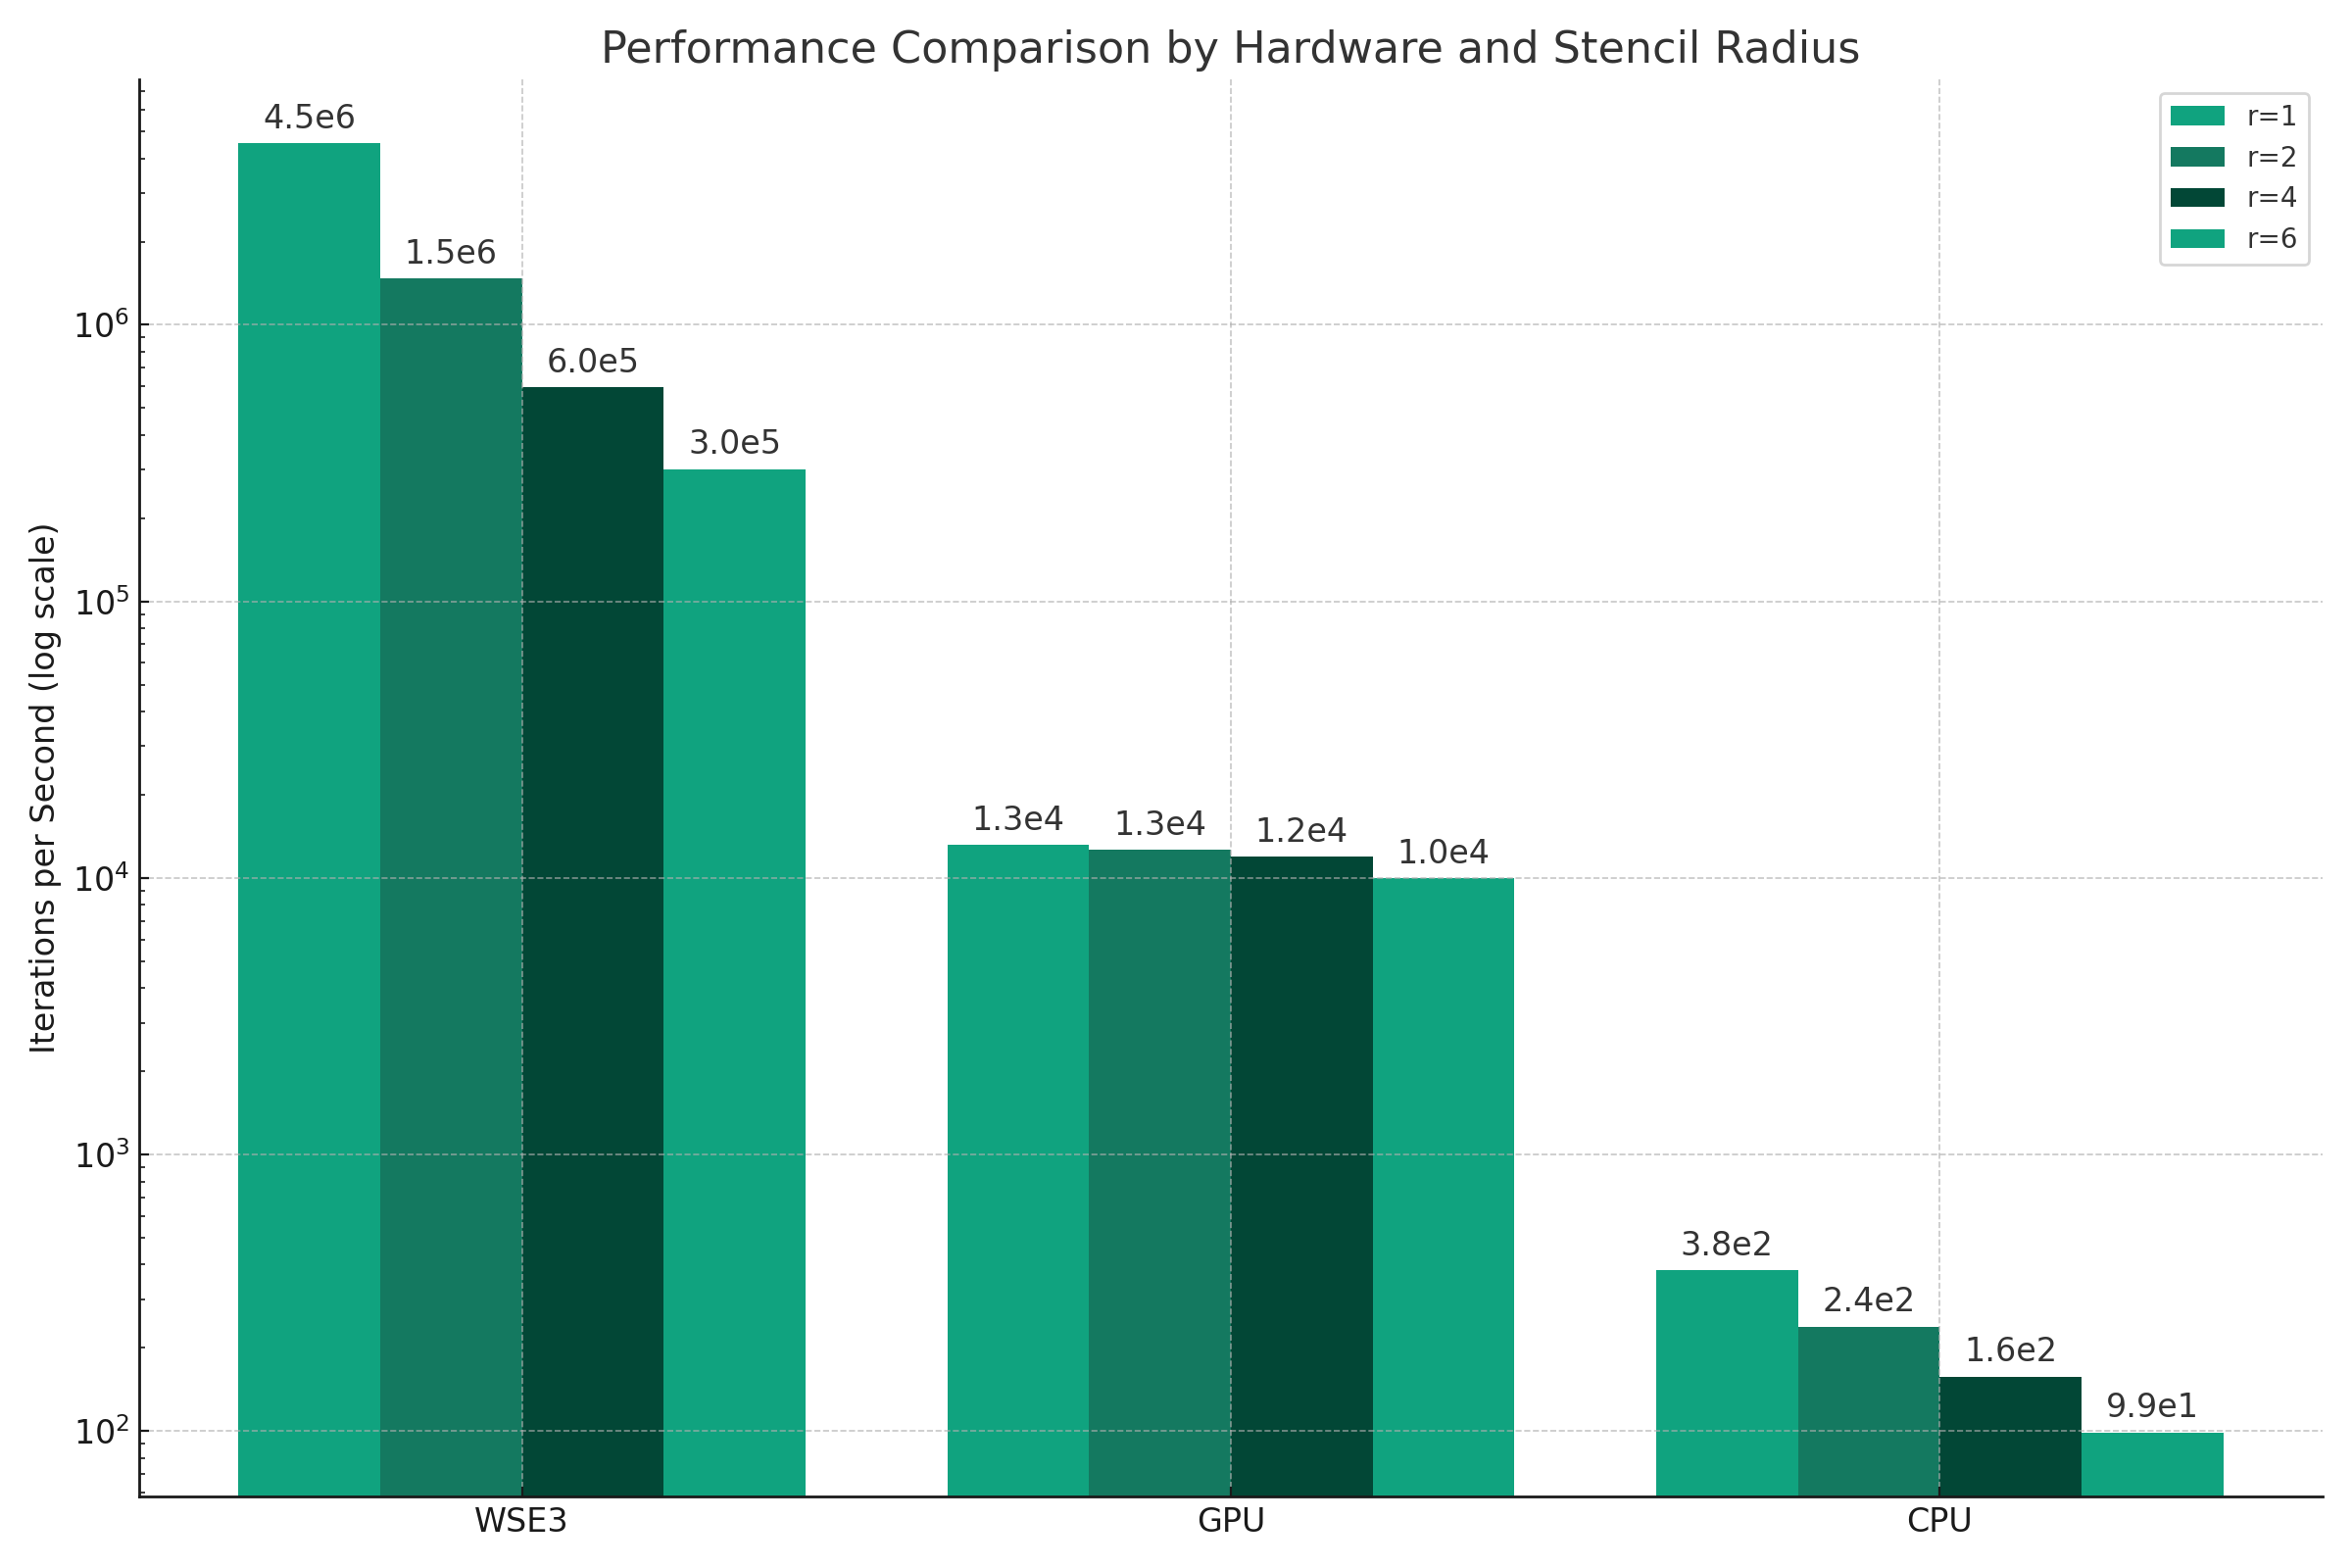
\includegraphics[width=0.5\linewidth]{cpu_gpu_cerebras_comparison.png}
%     \caption{Performance comparison across architectures for a $10^3 \times 10^4$ grid. The Cerebras \ac{wse}-3 implementation significantly outperforms the \ac{gpu} (NVIDIA H100) and \ac{cpu} (AMD EPYC 9554) across all radii. While the \ac{gpu} performance is largely insensitive to the stencil radius, indicating a memory-bound workload, the \ac{cpu} and \ac{wse}-3 performance degrades as the computational cost increases.}
%     \label{fig:cpu_gpu_cerebras_comparison}
% \end{figure}

% While the times for the \ac{gpu} and \ac{cpu} for this experiment where directly measured, we used the cycle count per iteration from the simulator for a significantly smaller grid size and a small iteration count, assumed perfect scaling to the full \ac{wse} dimensions as suggested from \autoref{sec:pe_overhead}, a constant cycle count per iteration and the clock speed of the \ac{wse} to calculate the time per iteration.

% The speedup for radius 1 from \ac{cpu} to \ac{gpu} is about 40x. From \ac{gpu} to \ac{wse}-3 we observe an even larger speedup of about 358x. As the problem is compute bound on cerebras while it is memory bound on \ac{gpu}, the speedup for radius 4 from \ac{gpu} to \ac{wse}-3 is significantly smaller at about 53x


To evaluate the performance advantage of the specialized non-tiled algorithm, we compare it directly with highly optimized implementations on traditional \ac{hpc} architectures using grid sizes that match the \ac{wse} dimensions. This comparison uses the actual \ac{wse} grid dimensions as the problem size, which represents the maximum grid size achievable with the non-tiled algorithm.

For \ac{wse}-2 with dimensions \numproduct{750 x 994} and \ac{wse}-3 with dimensions \numproduct{762 x 1176}, we measured the performance of the same radius-1 stencil on all three architectures.

\begin{figure}[h]
    \centering
    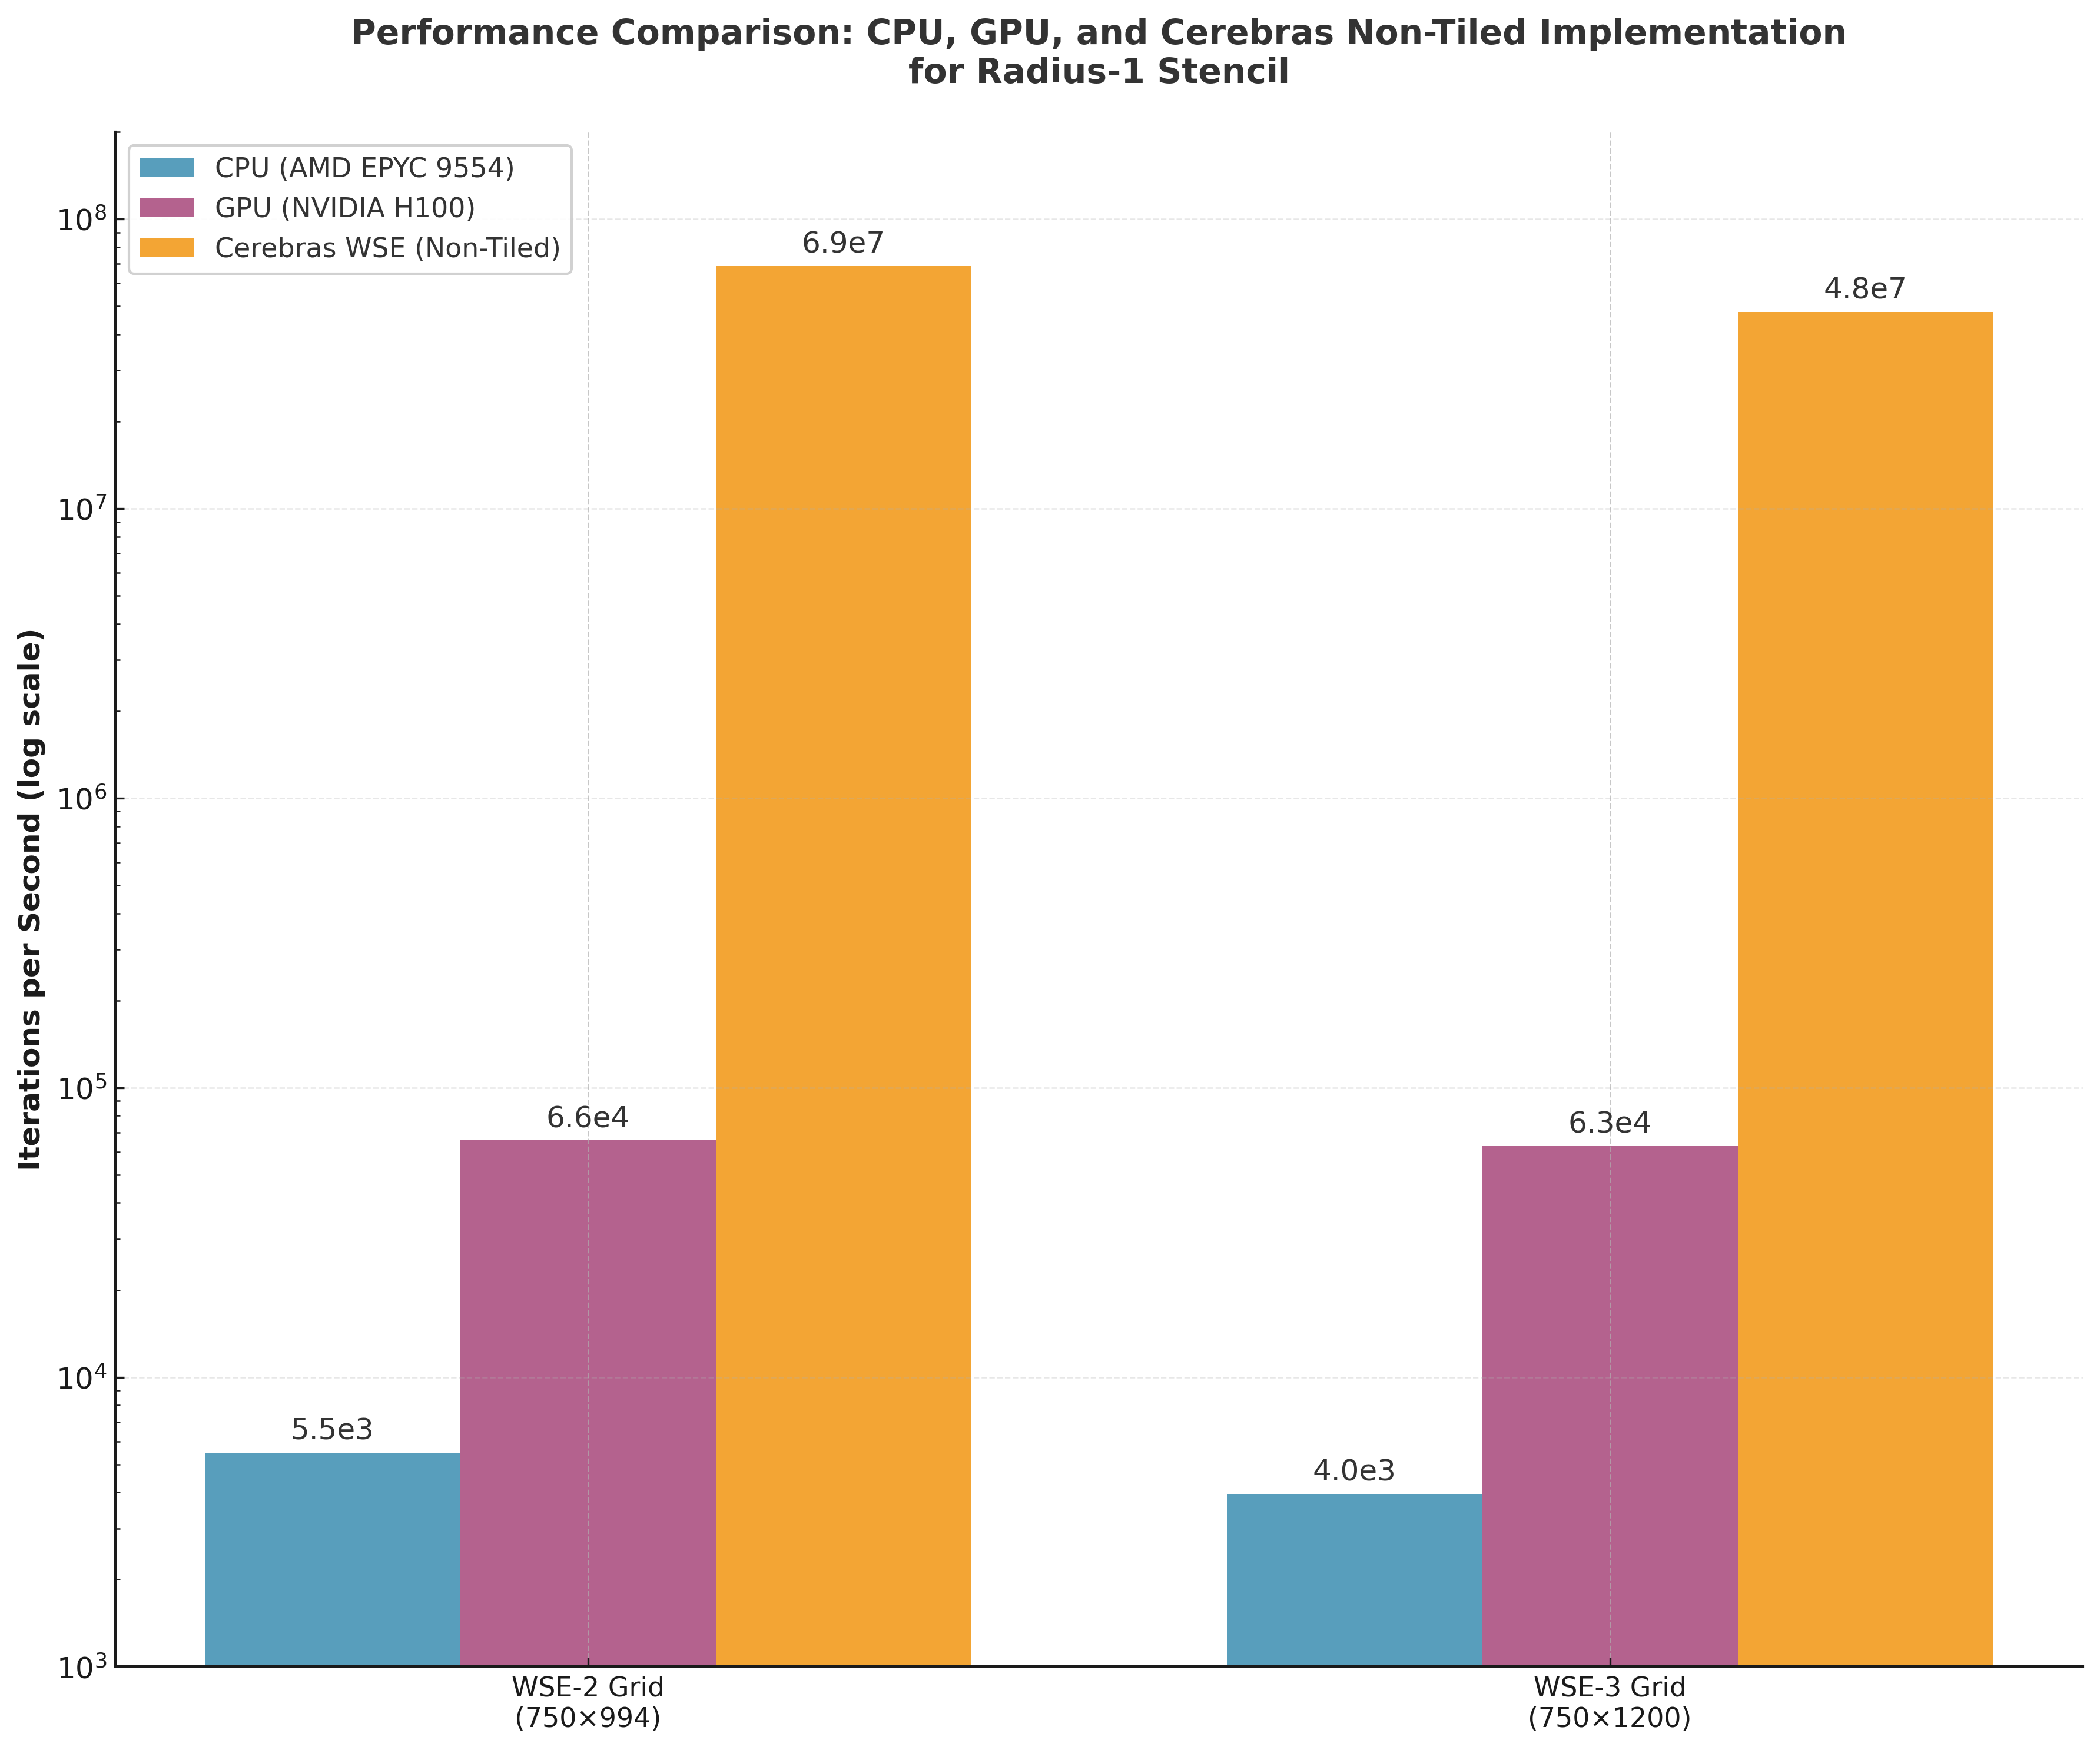
\includegraphics[width=0.7\linewidth]{cpu_gpu_cerebras_non_tiled_comparison.png}
    \caption{Performance comparison of the non-tiled Cerebras implementation against traditional \ac{hpc} architectures for radius-1 stencils. Results show iterations per second for grid sizes matching the \ac{wse} dimensions. The non-tiled algorithm achieves speedups of over 1000x compared to \ac{gpu} and over 12,000x compared to \ac{cpu}.}
    \label{fig:cpu_gpu_cerebras_non_tiled_comparison}
\end{figure}

The results demonstrate the exceptional performance of the non-tiled algorithm. For the \ac{wse}-2 grid size (\numproduct{750 x 994}), the Cerebras implementation achieves \num{68750000} iterations per second, compared to \num{65707} for the \ac{gpu}. This represents a speedup of 1046x.
For the \ac{wse}-3 grid size (\numproduct{762 x 1176}), the Cerebras implementation achieves \num{47826087} iterations per second, compared to \num{62743} for the \ac{gpu} with a speedup of 762x.

The performance advantage stems from the direct mapping of grid elements to \acp{pe}, enabling defacto in-memory computation with a memory that is significantly faster than the \ac{gpu} memory. While this approach is limited to grid sizes not exceeding the \ac{wse} dimensions, it provides unparalleled performance for problems that fit within these constraints.

\section{Percentage of peak performance}
Using the cycle counts per iteration from the simulator, we calculated the percentage of the \ac{wse}-2 and \ac{wse}-3 peak fp32 performance for different tile sizes and radii.
As described in \autoref{sec:implementation}, the non-tiled implementation and the r1-optimized implementation use \num{6} flops per grid element and iteration while the general tiled implementation uses \num{9} flops per grid element and iteration. From the respectively used tiled sizes in the different experiments, we first calculate the total number of flops per iteration and \ac{pe} and then divide by the measured cycle count per iteration to get an average flops per cycle and \ac{pe}. We find that the maximum number of fp32 operations per cycle and \ac{pe} can be obtained with \texttt{@fadds} instructions, which support a simd width of 2 in \ac{wse}-2 and 4 in \ac{wse}-3, while \texttt{@fmacs} is not supported in simd mode. Using the calculated average flops per cycle and \ac{pe} and the maximum flops per cycle and \ac{pe}, we calculate the percentage of the peak performance \autoref{fig:percent_pflops}.

\begin{figure}[h]
    \centering
    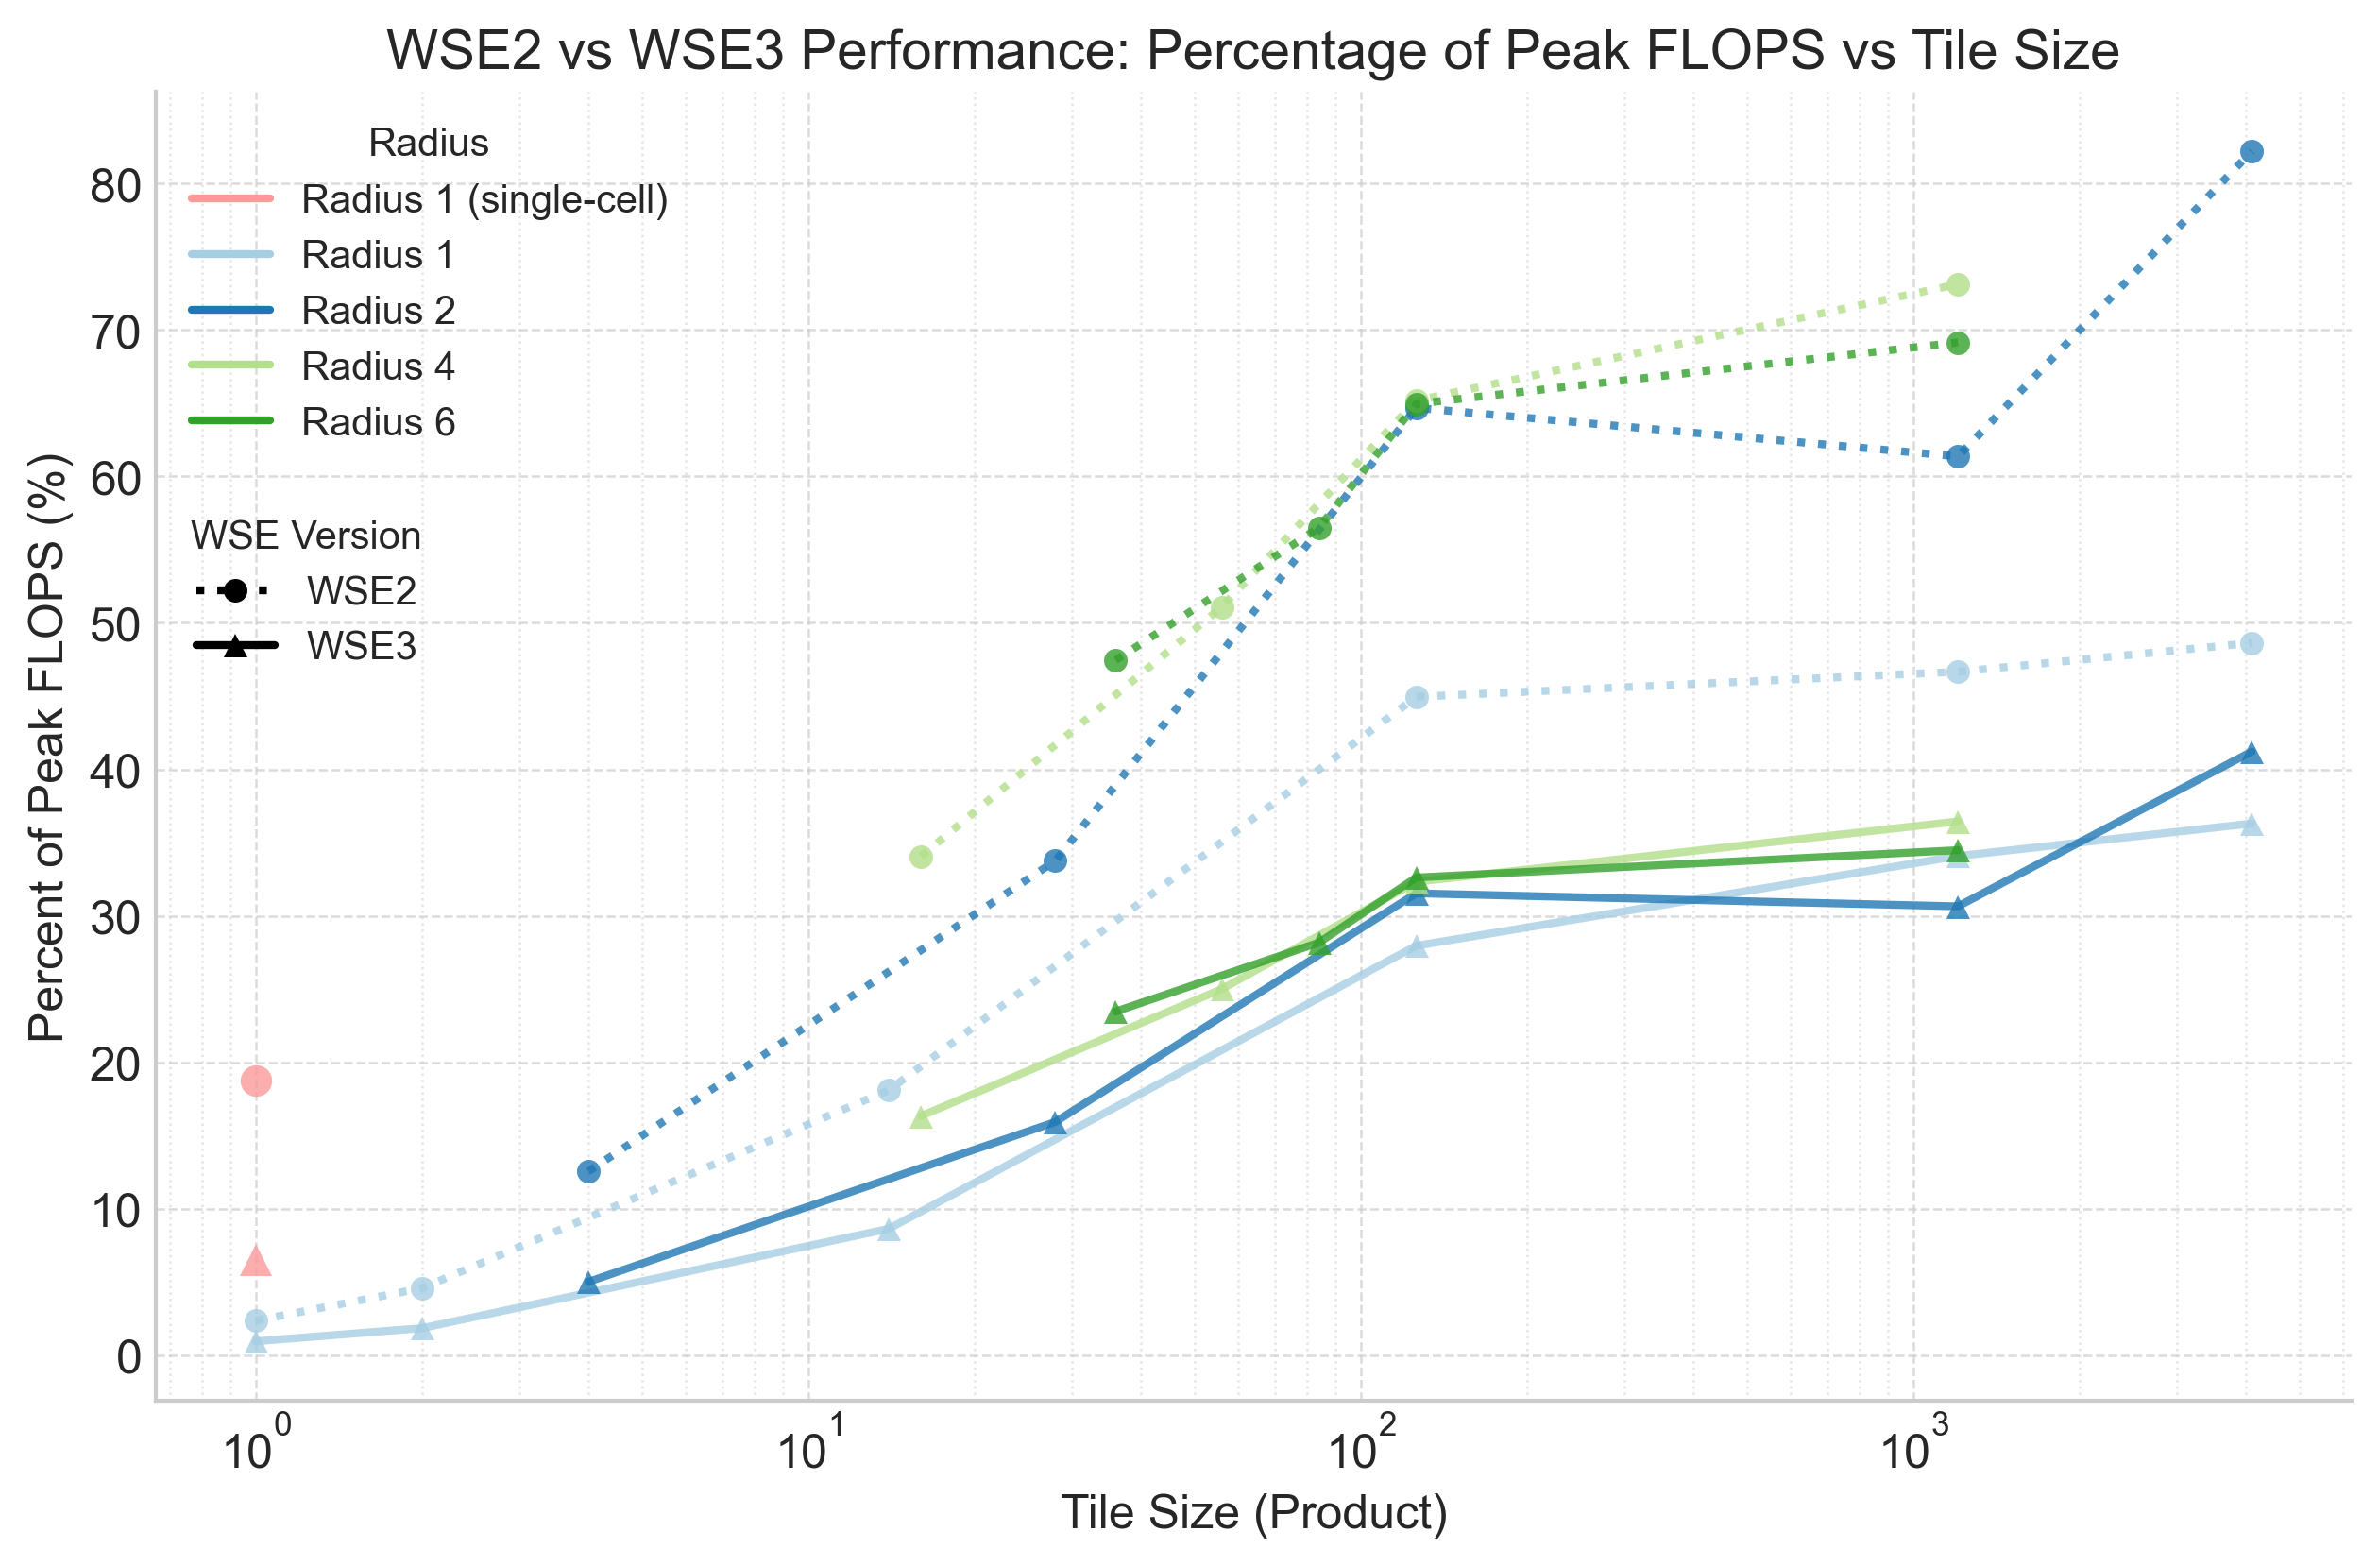
\includegraphics[width=0.7\linewidth]{percent_pflops.png}
    \caption{Percentage of peak performance for different tile sizes and radii for \ac{wse}-2 and \ac{wse}-3.}
    \label{fig:percent_pflops}
\end{figure}

For radius 1, and the maximum tile size of \numproduct{64 x 64} we reach \num{48}\% of the peak performance for \ac{wse}-2 and \num{36}\% for \ac{wse}-3.
While these numbers are per \ac{pe}, they also hold for the entire system, if the problem size is large enough to use the whole \ac{wse} dimensions.
In general, the archived percentage of peak performance mostly increases with the tile size and decreases with the radius.

In the optimal configuraion, our implementation reaches a sustained performance of 800 (797,6) TFLOP/s for \ac{wse}-2 and 1430 (1431,3) TFLOP/s for \ac{wse}-3.

\section{What contributes to the cycle count?}
We analyze the the instruction traces the simulator can record for what contributes to the the measured cycle counts.
We find that the effective simd width for some instructions in our implementation is lower than the theoretical maximum.
For \texttt{@fadds} it is 1.25 on wse-2 and 1.5 on wse-3.
The \texttt{@fmuls} instruction only have a simd width of 1 and we find that we measure exactly one cycle per instruction.

Here is a table that lists the different number of cycles per program segment. 